\documentclass[ twoside, openany, 12pt, a5paper]{book}
\usepackage{tikz}
\usepackage{Atlan}
\usepackage{pdfpages}
\usepackage{multicol}
\usepackage{geometry}
\usepackage{fancyhdr}
%\usepackage{ctex}
\usepackage{graphicx}
\usepackage{wrapfig}
\usepackage{tipa}
\usepackage{blindtext}
\usepackage{fontspec}
\usepackage{tabularx}
\usepackage{longtable}
\usepackage{tipa}
\usepackage[english]{babel}
\usepackage{lettrine}
\usepackage{wrapfig}
\usepackage{forest}
\usepackage{setspace}
\usepackage[style=authoryear]{biblatex}
\usepackage{multicol}
\usepackage[t,lf]{spectral}
\usepackage{xpatch}
\let\cleardoublepage=\clearpage

\newlength{\chaptertopskip}
\setlength{\chaptertopskip}{-50pt}
\makeatletter
\xpatchcmd{\@makechapterhead}{\vspace*{50\p@}}{\vspace*{\chaptertopskip}}{\typeout{Success}}{\typeout{Failure!!!}}
\makeatother

\addbibresource{./Bronnen/Atlan.bib}



\pagestyle{fancy}
\fancyhead{}
\fancyhead[LO]{{\fontsize{10}{12} \selectfont \leftmark}}
\fancyhead[RE]{{\fontsize{10}{12} \selectfont \rightmark}}  
\renewcommand{\headrulewidth}{0pt}
%%%%%%%%%%%Dependencies%%%%%%%%%%%%%%%
%\input{./Dependencies/Cmd}
%\input{./Dependencies/Grid}
%\input{./Dependencies/numberlines}

%%%%%%%%%%%Definitions%%%%%%%%%%%%%%%%
\def\Section#1#2{\section{#1}  \vspace*{-0.5cm} {\small \bf \begin{center} #2\end{center}}}


%%%%%%%%%%%Dimensions%%%%%%%%%%%%%%%%%%
\setlength{\footskip}{60pt}

\begin{document}
%%%%%%%%%%%%%%%%%%%%%%%%%%%%%%%%Frontmatter%%%%%%%%%%%%%%%%%%%%%%%%%%%%%%
\frontmatter
\documentclass[12pt, a5]{article}
\usepackage{graphicx}
\usepackage[lmargin=4cm,rmargin=2cm]{geometry}
\begin{document}

\thispagestyle{empty}
\setcounter{page}{-1}
\begin{center}
\includegraphics[scale=0.6]{../Images/LogoAtlan.jpeg}

\end{center}
\begin{center}
        \hspace{0.7cm}\resizebox{8cm}{!}{{\huge ATLAN}}

	
	\fontsize{21}{23}\selectfont \hspace{12.3pt}\fontdimen2\font=4.3pt Introduction\ to\ a\ proposed \\\hspace{0.5cm}philosophical \hspace{0.00cm}international \\auxiliary language
\end{center}


\end{document}


\chapter{Preface}



%Excerpt%%


\begin{center}{\it

	\includegraphics[scale=0.5]{./Images/Chinese.jpeg}



The Path that can be trodden, 

is not the eternal Path. 

The Name that can be named, 

is not the eternal Name. 

Nameless, it is the Originator  

of heaven and earth 

Named, it is the Mother  

of ten thousand things. 
}

...


-{\it Dao De Jing, chapter 1}

\end{center}



\hfill Ana Bosni\'{c}


\input{./Frontmatter/TOC.tex}

%%%%%%%%%%%%%%%%%%%%%%%%%%%%%%%%Mainmatter%%%%%%%%%%%%%%%%%%%%%%%%%%%%%%
\mainmatter

\chapter{Introduction}


\section{The story of King Atlas}




\section{Linguistic relativity \\ {\small Max Geraerdts}}


\section{Need for an IAL \\ {\small Jonathan Roose}}

\section{Eco's words \\ {\small Jonathan Roose}}


\chapter{Phonology}\Section{The Sound of Atlan}{Niek Elsinga and Stijn Janssens}



\chapter{Writing Atlan}\Section{Typography and direction of reading}{}
\lettrine{A}{tlan's} writing system is a natural application of our philosophy: start with elementary parts, and every complexity will be a mere combination of those parts. Our glyphs (as we shall call them) each denote one syllable. They always do so; they always will stand for the {\it same} syllable. Unlike English: in the words \lq\lq tone\rq\rq and  \lq\lq to\rq\rq, the \lq\lq to\rq\rq is pronounced respectively [t\textturnm] and [t\textbaro]. 

That is the rationale behind our writing system; let us dive into the details. As told, Atlan has a set of basic lines. They are:

\begin{center}

\begin{tabular}{c|c| m{1cm} |c}
\hline
\multicolumn{2}{c}{Consonants} & \multicolumn{2}{c}{Vowels} \\ 
\hline
{\bf Line} & {\bf In I.P.A.} & {\bf Line} & {\bf In I.P.A.} \\
\DeclareStroke{\CenterVertical} & ... & \Atlanu & ... \\  
\hline
\DeclareStroke{\CenterHorizontal} & ... &  \Atlani & ... \\ 
\DeclareStroke{\BigNW} & ... & \Atlana & ... \\ 
\DeclareStroke{\BigSW} & ... & \Atlano & ... \\ 
\DeclareStroke{\BigSE} & ... & \Atlane & ... \\
\DeclareStroke{\BigNW} & ... & & \\
\DeclareStroke{\Dot{Center}} & ...& &\\
\DeclareStroke{\MediumCircle{Center}} & ... & & \\
\end{tabular}

\end{center}

These lines all represent a single vowel ({\it V}), or a single consonant ({\it C}). We can combine them to make syllables. By combining two consonant lines, you get a CVC-syllable, such as {\it loj}, {\it pas} or {\it mup}. You can also make a VC-syllable, such as {\it mu}, {\it po}, or {\it ji}. The vowels don't have separate lines in a CVC or VC-syllable; instead, the vowel is determined by the position of the two consonant-lines. We will go deeper into that below. First, we give the rules for the order of the consonants and vowels: what determines whether two lines make e.g. {\it poj} or {\it jop}, {\it mu} or {\it um}? 

This order is determined by the manner in which the lines combine. There is always a \lq\lq bigger \rq\rq line, and a smaller one. These lines fit inside an imaginary box. The position of the smaller line relative to the bigger line, determines the order of consonants. A general rule of thumb is best given with the help of a box:

\begin{center}

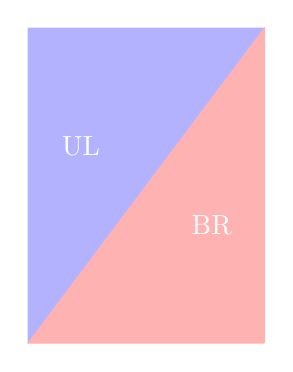
\begin{tikzpicture}
\draw[blue!30, fill= blue!30] (0,0) -- (3,4) -- (0,4) -- (0,0);
\draw[red!30,fill =red!30] (3,0) -- (3,4) -- (0,0) -- (3,0);
\node(A) at (0.67,2.5){\color{white} UL};
\node(B) at (2.33,1.5){\color{white} BR};
\end{tikzpicture}

{\it \footnotesize Figure 1: Box for determining consonant order.}
\end{center}

If the smaller line is in the upper-left triangle (UL), it the consonant it designates comes first. If it is in the bottom-right one, it comes second. For the rest of the explanation, it is advised to keep this box in the back of your head. An example:

\def\restorecorps{\renewcommand{\corpsgrootte}{20pt}}
\begin{wrapfigure}[7]{l}{0.4\textwidth}
\renewcommand{\corpsgrootte}{100pt}
\kus
\restorecorps
\end{wrapfigure}

As you see here, the smaller line is found on top. Hence, it is placed inside the upper-left triangle. The consonant for which the smaller horizontal line stands (the {\it k}), comes before the other consonant, the {\it s}.

\phantom{}

\begin{center}
\definecolor{melon}{RGB}{255,179,179}
\definecolor{caian}{RGB}{204,255,247}
\definecolor{lavender}{RGB}{242,179,255}
\definecolor{jasmine}{RGB}{255,212,128}
\definecolor{lemon}{RGB}{255,247,204}
\begin{tikzpicture}
\draw[black] (0,0) rectangle (3,4);
\draw[fill = melon] (0,4) rectangle (3,3.5);
\draw[fill = melon] (0,0.5) rectangle (3,0);
\draw[fill = melon] (-0.25, 0) rectangle (0,4);
\draw[fill = melon] (3.25, 0) rectangle (3,4);
\draw[fill = caian] (1.5,2.5) rectangle (0,3.5);
\draw[fill = caian] (1.5,2.5) rectangle (3,3.5);
\draw[fill = jasmine] (1.5,1.5) rectangle (0,0.5);
\draw[fill = jasmine] (1.5,1.5) rectangle (3,0.5);
\draw[fill = lemon] (1.5,1.5) rectangle (0,2.5);
\draw[fill = lemon] (1.5,1.5) rectangle (3,2.5);
\draw[fill = lavender] (1.5,2) circle (0.5);
\node at (1.5,3.75){u};
\node at (0.75,3){i};
\node at (2.25,3){i};
\node at (0.75,2){a};
\node at (2.25,2){a};
\node at (0.75,1){o};
\node at (2.25,1){o};
\node at (1.5,0.25){u};
\node at (1.5,2){e};
\node at (-0.375, 2){\footnotesize u};
\node at (3.125, 2){\footnotesize u};
\end{tikzpicture}
\end{center}

The vowel is...
\begin{itemize}
\item {\it u} if the smaller line is found at the edges. The smaller line is in its whole above, under, left or right of the main line. 

\item {\it i} if the smaller line is found on the upper-left or upper-right side of the main line. It is usually smaller than the line made for {\it u}, to avoid confusion. 

\item {\it a} if the smaller line is found left or right to the middle of the line. 

\item {\it o} if the smaller line is found on the bottom-left or bottom-right hand of the main line. Again, this line is smaller than the line for {\it u}. 

\item{\it e} if the smaller line is placed in the middle. Or, if the small line intersects with the main line at the middle. In some instances, the small line is then split up by the main line.  
\end{itemize}

Then we have a single exception. You can combine two equivalent lines, to make syllables such as {\it pop}, {\it mum}, or {\it lol}. The order of these lines doesn't matter; hence we choose place the smaller line to the upper-left of the main line in such cases. For the vowel {\it u}, there are two small lines, split at the center. For {\it e}, there are either two or three small lines. At least one of those lines crosses through the center of the imaginary box.
%EXAMPLE>?

Remember that the {\it p} is represented by the dot \DeclareStroke{\Dot{Center}} . For clarity, we couldn't combine simply two dots to make a full syllable. Hence, 


These are the rules. 

\Section{Numerals and Mathmatics}{}


\Section{Font in \TeX}{Jarno Smets}


\Section{On Dyslexia}{Stijn Janssens and Jonathan Roose}

\Section{Cartouche}{}




\chapter{Morphosyntax}
\Section{Unambiguous Syntax}{Jarno Smets}


\chapter{Our Ontology}%%Introduction

\lettrine{T}{he} goal of this is to expound on the ontology of the language, which concerns its semantics and syntactical inventory. I will achieve this by discussing the literature on various attempts and classifications proposed within the topics, and then dividing all linguistic meaning into its irreducible, unambiguous and unique atomic components, as to respect constraint 2 (unambiguity). It will use some principles of natural bifurcation of meaning (5.1.2), and built off of the universal substratum of phenomenology and qualia (5.2 and 5.3). It will also be linguistically grounded in the culturally universal basic elements of human life (5.4).


\section{Parsimony in semantics}

\subsection{\it Oligosynthesis}


Besides constraint 1 (cultural neutrality), which will be discussed in chapter 5.4, Atlan’s lexicon has to follow constraint 2 (unambiguity) and 3 (parsimony), which will be discussed in this section. Ideally, the language should contain as little basic words as possible, as to reduce the time required to learn the language. Therefore, it should be sparse with its words, only adding new words when these carry a meaning that is not already covered by another word. Complex concepts should not get their own separate words, for this would add an inestimably large number of extra words, but rather be composed of more simple and universal words that constitute its meaning. Atlan shall achieve this by using a semantic system that is oligosynthetic, meaning that it has a very limited number of semantic atoms\footnotemark (\textit{oligo}  = few), from which more complex meaning is built by combining different atoms (\textit{synthesis}  = combining). Each semantic atom (or ‘root’) shall be covered by a unique one-syllable word. Atlan syllables can take four shapes (C = some consonant, V = some vowel): V, CV, VC, CVC. This is abbreviated to (C)V(C). There are 9 consonants and 5 vowels in its phonetic inventory, yielding a total of 5 + 5x9 + 5x9 + 5x9x9 = 500 possible combinations, however all syllables ending in \textit{-ij} cannot be sufficiently distinguished by ear from those ending in \textit{-i}, so all (-) \textit{ij} will not be included. This leaves a total number of 490, and thus the challenge posed in this chapter is that of reducing all meaning to 490 atoms or a combination of these.  

\footnotetext{Throughout the book we refer to Atlans syllable words as 'semantic atoms / primes', but this definition is roughly equal to the linguistic term 'morpheme', which means as much as 'the smallest unit of meaning'. Since the atoms play a crucial role in Atlan's oligosynthetic structure, and this is not covered by the term 'morpheme' alone (which also doesn't neccesarily have to be a single syllable), we opt for this specified terminology.}

The term \textit{oligosynthetic} was first coined by the linguist Benjamin Lee Whorf and is defined as having at most a few hundred-word roots. However, this seems to be extremely rare among natural languages. A possible example might be the Kalam language of the Highlands of New Guinea (Pawley A. , 1993). Two other languages previously regarded as oligosynthetic by Whorf are the Aztec language Nahuatl and the Native American language Blackfoot, but these are now commonly classified as polysynthetic (using many roots to synthesise more complicated meaning). Oligosynthesis is more popular among constructed languages, such as Sona, Ro, aUI, Ygyde and Kali-sise (FrathWiki, Oligosynthetic language, n.d.). These all have different numbers of semantic primes and methods of synthesising them, but they commonly have the following problems (Watson, n.d.): 

\begin{itemize}
\item [I.] Complicated combinatory systems  

\item[II.] Unclear word-parsing  

\item[III.]Vagueness of composite meaning 
\end{itemize}

Atlan will overcome problem I by using an extremely basic manner of combinatory synthesis: the most semantically essential prime comes first and is followed by primes that hierarchically specify the meaning of the word. Grammatical functions always come in front of the semantic root as prefixes (except for the plural1), and semantic specifications are appended as suffixes. Atlan's word-composition is as follows:  

\begin{center}
{grammatical.function –  main.semantic.root – semantic.specification – plural} 
\end{center}
\quad
 

This will also solve problem II, because syllables can be recognised to be semantic when they are CVC, and grammatical otherwise. This way, grammatical syllables are easily distinguished from semantic ones. It is therefore always audibly clear where a word begins and ends. In written text this is aided by the fact that in Atlan’s own writing system, CV and VC syllables always consist of a small circle attached to a line, while CVC syllables are always two lines connected to each other.  

The 5 V syllables will be restricted to mood-markers and general sentence structuring, because of the onomatopoeic quality of these basic vocal sounds. These, however, can also be used grammatically to modify the meaning of nouns, verbs and pronouns, for example to turn ´here´ into ´where?´.  
\begin{itemize}
\item    Exclamative (prosody), imperative, vocative = o  \Atlano

\item    Interrogative (question, prosody) = e  \Atlane

\item    Stress marker (prosody) = a + stress \Atlana

\item    Relative clause = i (+ pronoun) \Atlani

\item    Subjunctive (wish) = u \Atlanu
\end{itemize}

 

The 89 CV, VC syllables will be mostly restricted to morphological and abstract functions, indicating grammatical, syntactical or logical functions and relationships between words. Logical functions will be derived from the logical operators of predicate logic and possible worlds semantics (Priest, 2011), and grammatical functions are derived from the Universal Networking Language (UNL) (Portal, sd), and syntax-semantically reduced where possible (see chapter 6.2). UNL was initiated by the United Nations University in 1996 and continued by the international non-profit organisation UNDL from 2001 onwards. Its goal is to function as a formalised pivot language between natural language and interlingual machine translation, therefore having formalised all grammatical functions, together with a large-scale ontology of all concepts contained within all its source languages (Universal Networking Language Portal, n.d.). Atlan does not use the latter, however, because it would break constraint 3, parsimony. 	

The remaining 396 CVC syllables will cover the semantic primes, and these will be systematically selected and ordered in the remainder of the current chapter and chapter 3 and 4. Because Atlan’s writing system is syllabic, and each syllable has a fixed semantic value assigned to it, individual glyphs can be read both phonetically as well as ideographically/logographically. This would allow for it to be a kind of interlingual orthography. 

Problem III, that of vagueness of composite meaning, will be tackled in several ways. Most importantly, some of the most universal ‘semantic molecules’ (see chapter 3) will have their own assigned syllable. These molecules are definitions that could be reduced to more fundamental atoms but are often used to build more complex meanings, therefore being condensed into a molecule as to prevent unnecessary complexity of compound words. However, this is not an all-encompassing solution for words that have very specific and context derived definitions. 

{\it Circumlocution} is the phenomenon where concepts which do not have a specific word for them in a language are described by giving a circuitous description of the intended meaning. An example of this in English would be ‘the day after tomorrow’. Atlan will never be able to fully eliminate some forms of circumlocution in its lexicon, mainly because of it being an oligosynthetic language. However, confusion around these instanced can be minimalised in the following ways.  

A standardized set of compound definitions can aid speakers by being a guideline to using compound words. Someone who learns the language, would have to learn the 490 semantic primes, and then be familiarized with some standardized compound words. Because the meaning of the compound word will be derived from the syllables it contains, learning these compound words will be intuitive and require less mnemonic effort than learning a completely new word would. This way, when a speaker encounters a word they have never heard before, they will be able to derive, or at least estimate the intended meaning just by recognizing its syllables.

Additionally, neologisms could be created during improvised language use, as a sort of generative etymology, and be directly perceived by the listener, possibly allowing for freer linguistic cultural- and self-expression. Finally, some compound words will be systematically constructed in a taxonomical fashion, when the word’s definition allows for this, such as is the case for all living creatures. Each compound word is sorted along the axis of importance, with the most fundamental semantic prime in front, and followed by other primes that hierarchically add layers of semantic precision. This creates a universal logic in the composition of compound words that allows one to identify the ontological category in which the word falls and refine the definition by the refining descriptors appended to it, as if ‘zooming in’ with a semantic lens.


\subsection{Taxonomy}

\vspace{0.3cm}
\begin{center}
\includegraphics[scale=0.5]{./Images/tree.jpeg}

{\footnotesize \it Tree of Porphyry, taken from Cohen (2007)}
\end{center}

\noindent Many philosophical constructed languages that came before Atlan suggested or employed a so-called taxonomical ontology. Many of these are inspired by a diagram invented by the 3rd century Neoplatonist Porphyry when explaining Aristotle’s Categories (Porphyry, 300), called the Porphyrian tree (Franklin, 1986). In the Categories, Aristotle outlines a broad ontology of human apprehension, classifying everything that can be the subject or predicate of a statement into 10 categories: substance, quantity, quality, relation, place, time, position, state, action, affection (Aristoteles, 40). The Porphyrian tree (shown below) shows how a human falls into these categories, by showing different bifurcations from the first five categories (Cohen, 2007): 

Before Aristotle, similar ontological categorisations were made by the Vaiseshika school (Padārtha) (Stanford University, 2019) and the Stoic school, and after him numerous other thinkers, including Plotinus (430, 2019), Kant (Categories) (1781, 1998), Hegel  (1812, 1975), Peirce (1867), Husserl (1900, 1993) and Whitehead (categorial scheme) (1929, 2010). Not to mention folk ontologies, such as the Bantu nominal classes (Bleek, 1862–69) and the common distinction between animate and inanimate. All of these mostly were not taxonomical, however, and have been discussed extensively, but it is not the purpose of this paper to further investigate these discourses.  

\phantom{.}\\

There is, however, one specific notion within these categorisations which Atlan will incorporate, namely that of the {\it triadic categorisation} of Being. In Hegel, this comprises 1) Being (mind, consciousness, sensation), 2) Essence (Other, duality) and 3) Notion (synthesis, reference). In Peirce, these equate to Firstness (Quality, feeling, consciousness), Secondness (Reaction) and Thirdness (Meaning, representation). Atlan incorporates this through three degrees of removing from the speaking subject (see chapter 6.2). The first degree can be combined with the semantic prime for ‘person’ (´EJ´ \ej) to mean ‘I’ (´EJ.AM´ \ej \am), the second degree to mean ‘you’ (EJ.UN \ej \un) and the third to mean ‘he / she / they’ (´EJ.AJ´ \ej \aj), as well as other primes like place, time and demonstratives. 

\vspace{-0.1cm}
A more explicit taxonomical ontology makes use of a so-called hierarchical classification. The idea of a ‘perfect’ or philosophical language was a popular idea during the enlightenment, being discussed by Bacon, Descartes, and Newton as a part of a widespread desire for a language that does not confuse the speaker’s understanding of reality or distort the natural order present in it (Eco, 1994, pp. 209-227). 

The core idea of such a language is that it would build its words by adding different letters for every hierarchy of meaning. This way, related words would sound similar. There is, however, always a necessary degree of arbitrariness to such a system, since the arbitrary choice has to be made of what categories are specified by adding a limited set of different letters. These would have to be made from scratch, not based on previous languages, as to avoid confusion caused by natural language. These languages are known as a priori, and Atlan will be a priori as well, even though its contents are sourced from data from many natural languages but recombined in an attempt to circumvent natural language confusion.  

The first serious attempts at this ideal were made by George Dalgarno in his {\it Ars signorum} (1661, 1968) and John Wilkins in his \textit{Essay Towards a Real Character and a Philosophical Language} (1668, 1968). Initially, the two collaborated on a philosophical oligosynthetic language, but they couldn’t agree on whether to make the taxonomy encyclopaedic or build compound words from a small set of primes. Wilkins published his own version based on the former and Dalgarno the latter. Dalgarno’s language sadly never caught on, perhaps because the explanation of the linguistic working of the language was shrouded in philosophy which explained the structure \footnote{We hope this is not the case for this book as well.}. 

Wilkin’s language found a bit more recognition, being originally taken seriously by the Royal Society, with an attempt to finish the language after his death by a designated committee. It too, however, slowly lost interest in people and descended into oblivion  (FrathWiki, Ars Signorum, n.d.). Its taxonomical classification was structured to encompass every animal, plant, mineral and artifact. He achieved this by setting up an ingenious taxonomical tree to indicate the relations and bifurcations of meaning, along with a system of hierarchically adding vowels and consonants to specify differences and species within different categories. 

Wilkins regarded the language presented in his essay as just a draft, although he provides 2,030 different primitives, as well as a 15,000-word list for different English words but admits that it should be worked out by different teams of scientists to work out different concepts within their respective disciplines. His collaboration with the Royal Society was largely part of that attempt. Later on, Wilkin’s taxonomy went on to inspire Roget’s Thesaurus (1805) and later on Diderot and d’Alembert’s Encyclopaedia (1759).  

The idea was met with criticism as well. Voltaire criticised the optimism of the people attempting to create such a language in the form of the character Dr. Pangloss in his satire \textit{Candide} (1759, 1963). Jorge Luis Borges wrote an essay criticising taxonomical categorisations in general and Wilkin’s language specifically (1942) in which he mocks different instances of arbitrary classification by mentioning a fictional Chinese taxonomy called the \textit{Celestial Emporium of Benevolent Knowledge}. This list contains some very culture-specific, arbitrary and absurd categories such as ‘those belonging to the Emperor’, ‘those that have just broken the vase’ and ‘those that from afar look like flies’. This criticism seems like a bit of a stretch, because Wilkins put in a systematic effort to make a coherent classification, and this is not as arbitrary or absurd as Borges’ fictional classification. 

The linguist George Lakoff supports this claim by stating that many non-western cultures use classifications similar to European ones (Lakoff, 1987). Borges does point out that a successful execution of the idea could in theory have many benefits: ‘‘Mauthner points out that children would be able to learn this language without knowing it be artificial; afterwards, at school, they would discover it being an universal code and a secret encyclopaedia’’ (Blevins, n.d.). 

Foucault was inspired by Borges’ essay to write his book \textit{The Order of Things} (1966, 2010, preface) in which he analyses the social grounding of epistemic assumptions. He argues that implicit norms within intellectual communities determine thought and influence which topics are researched, and which are not, and how the established bias influences the interpretation of the data that is found. These assumptions and norms are bound to cultural and historic settings, and periodically go through reforms as a result of paradigm shifts. This is a strong blow to the aspiration of a universal classification of the universe. Borges claims that this is because: ‘‘we do not know what sort of thing the universe is’’. Metaphysicians and phenomenologists might differ on this, however, as will be discussed in chapter 3 of this essay.  

Besides this, Wilkins’ system has the disadvantage of only having a limited number of differences and species that can be specified because of the limited phonology. Atlan will be more similar to Dalgarno’s language, in that it will not drive its words through a hierarchical process of taxonomy, but rather by combining primes at will, allowing for exponentially more semantic combinations than are possible in Wilkin’s system. 

Another problem of Wilkin’s language is that words with similar meanings have very similar pronunciations, to the point of confusion. Modern information theory warns of this (Norman, n.d.), and Eco even identified that Wilkins himself made such a mistake, confusing {\it Gade} (barley) for {\it Gape} (tulip) (1994, p. 249). This would hinder the language’s intelligibility when mishearing can easily change important nuances in definition, as well as making is harder to speak fluently, because any speaker would have to work through tables and flowcharts in their minds while simultaneously talking, without making any mistakes. The language would also be very intolerant of subtle shifts in pronunciation and phrasing that tend to occur naturally within languages over time, because this would cause the whole encyclopaedic house of cards to come crashing down. 

Atlan will not have this problem, because its semantic primes are syllables instead of phonemes, and Atlan’s phonemic inventory is built to accommodate variation in phonetic approximation and sound shifts within its 14 archetype letters, without causing confusion or ambiguity. 

The philosopher Deleuze and psychoanalyst Guatarri proposed an alternative to arborescent (tree-like, hierarchical) epistemic networks like employed by Wilkins and Dalgarno, namely that of a {\it rhizome}, an analogy with a decentralised plant root network (1980, 2019). Such a model does account for bifurcations and conceptual relatedness but is more modal and allows for more complex interlinking than mere hierarchy. It would also fit the philosopher Quine’s idea of an interrelated epistemic ‘web of beliefs’ (Ney, 2014), as well as Wittgenstein’s claim that concepts are not clearly delineated, but rather surrounded by a ‘corona’ of associated concepts (1953, 2010, p.181). 

Because of this, the main ontology seems to be better off using a combinatory system, which would allow for endless recombination and web-like relationships between similar words. This however doesn’t mean arborescent taxonomy should be completely abandoned. The most relevant modern case of taxonomical classification is that of natural species, although individual species don’t have clear demarcations and are loosely defined by their ability to produce fertile offspring (Nature Publishing Group, n.d.). Genetic diversification happened through bifurcation, known as {\it speciation}. The reverse, different species merging into one through hybridisation, called {\it despeciation}, does sometimes occur (including among early hominins), but is exceedingly rarer (Junior, 2018). Because of this, the evolutionary tree of life is primarily arborescent. 

Modern biological taxonomy employs the following hierarchical classification: life – domain – kingdom – phylum – class – order – family – genus – species (Biology Dictionary, 2017). Atlan’s biological lexicon is constructed along this framework, using semantic primes to describe different bifurcations, inspired by the Latin etymologies employed in binomial nomenclature (a hangover from Latin being the academic {\it lingua franca}). These binomial nomenclatures only mention genus and species names of an organism, and words to designate species can re-occur in other genera to identify other species, adding to the parsimony of terms required to name all creatures within this system. 

Atlan shall have separate primes for the categories: \textit{virus, bacteria, archaea, plants, amoebas, fungi, animals.} In chapter 4 of this essay, a few culturally universal animal terms are identified, and these will be reduced to: \textit{mammal, fish, bird, worm, reptilian, insect.} Other animals could be reduced to their descriptions: sponges could be designated as foam-animals, starfishes to star-animals, snakes to legless-reptiles, amphibians to mucus-reptiles, molluscs to shell-animals, jellyfish to mucus-animals etc.  


Chemical molecules could be named by formalising a translation of the IUPAC nomenclature of organic chemistry from the originally Greek roots (IUPAC, 2021). Just like Wilkin’s language, Atlan will be dependent on scientists and specialists of different kinds of professions to add formalisations of their respective jargon nomenclatures to the lexicon in order to fully flesh out its lexicon. 

The reason why such a systematic description of reality claiming to be universal might be problematic, could be that it claims to have an objective image of reality, while all human thought, individual or collective, will always be fundamentally sourced from subjective experience. The philosopher Thomas Nagel described this by saying that there is no \textit{view from nowhere}\ (1989), while such a taxonomy appears to claim this anyway. The fact is that human concepts always have a necessary degree of arbitrariness because of the limited resolution of our conceptual boundaries. A taxonomical ontology implies the possibility of grasping some fundamental reductionist principle inherent to reality, while failing to see that many human concepts are emergent phenomena. The linguistic concept of an ‘organism’ cannot be reduced to a collection of organic molecules, because it is their complicated interplay that generates the multiple properties that pertain to an emergent system of self-preservation that humans call a single organism (Brigandt \& Love., 2017). On a microscopic level however, the clear boundaries of any single individual become fuzzy. It is because human life does not generally take place within a microscopic paradigm, that our concepts don’t have this level of detail. Reality is never described objectively, but always relative to the individual(s) observing and describing their reality. Humans appear to be ‘at the centre’ of their own language and understanding of reality. 

\section{The anthropocentricity of language}

Language and ontology are strongly entwined with one another: an ontological system is dependent on the words available to name its parts, and likewise a language is built from the set of concepts, relations, abstractions and ‘things’ that are captured by its lexicon  (Moltmann, 2017) (Boucon, 2019). Though by far not being the only elaboration on this idea, the Sapir-Whorf hypothesis is the most well-known inference that has been drawn from it. In short, this idea postulates that the range and limits of a person’s thought are determined by the language they speak. The strong version of this claim, linguistic relativism contends that all of human thought is fundamentally determined by language (linguistic determinism), resulting in some thoughts being lost and modified through translation or even untranslatable. It treats language as a fixed set of cognitive tools that acts as a constraint on the individual. This view, however, doesn’t enjoy a scholarly consensus (Whorf, 1956).  

However, this conception of language seems to be monolithic and extra personal instead of dynamic and dependant on individuals and their fluid interactions. It is challenged when presented with the fact that people within the same language can have vastly different ontologies, philosophies and vocabularies, depending on their individual personalities, interests and social environment, and the fact that individual people can learn multiple different languages and express their thoughts through them, nonetheless. Multilingualism is, however, noted to create within an individual, multiple linguistic ‘personæ’ for the different spoken languages, where one’s way of formulating thoughts and uttered sentences are altered by the individual characteristics of the different languages  (Pavlenko, 2006). 

Perhaps the influence that language has on the thoughts of a speaker can be likened to how putting on different glasses can alter one’s perception but does not change the fundamental scene being perceived through them. Sunglasses block out UV light, tinted glasses block out certain colours, different lenses shift the focus to what is near and other to what is far etc.: they all suppress some elements and amplify others, but they never change the basic composition of what is being perceived (if we discount virtual reality glasses). 

Using this metaphor, the purpose of Atlan is somewhat similar to being a clear, untainted, undeformed, unbiased pair of linguistic glasses, for as far as this is possible. Every single person’s eyes are different, and the glasses of their native language might be more or less similar to Atlan’s. The question then becomes: what constitutes this clear human experience that becomes tainted by language?  

First, we must realise that language itself is ontologically dependant on the total sum of living speakers. A dead, forgotten or undeciphered language cannot be said to currently exist in the same way that a living language like English exists. It might be revived in the future through the reconstruction of its linguistic information, but it only comes back into being when living humans are again able to read, write or speak the language. Furthermore, Wittgenstein’s private language argument states that a language is a fundamentally social thing, and that a purely personal language is therefore by definition impossible (1953, 2010, \S 243-271). Language is a complicated system of communicating all kinds of mental information, like thoughts, feelings, intentions, physical data \&c., for all kinds of different purposes, like cooperation, social bonding, problem solving . In individual growing up in solitude or alongside animals never has the need nor possibility to learn and use a language, because there are no other humans around to converse with. After having passed the critical period of language acquisition without ever having learned a human language, an individual will never again be able to do so later in life (Robson, 2002).  

Therefore, language is an inherently human thing, that emerged from the transferring of information from one person’s individual experience to another’s. Phenomenal cues, like the sound of words, the rhythm of speech, facial expressions and gestures are used as an interpersonal bridge between the private mental worlds of the separate individuals. Someone can both hear themself talking, as well as someone else: language exists in a shared phenomenal space, whereas inner thought is private. Language then becomes a highly codified system of phenomenal metaphors. The sound of a specific word is not the same as the information it codifies, but is consistently associated with the referred phenomenon, in the form of an abstracted ‘concept’. 

Atlan should thus have an ontology that is built off the subjective human experience, when regarded in a social context and in direct contact with its physical environment. This immediately brings a degree of anthropocentricity with it, because words relating to the human psyche, body, daily life, social environment etc. will be given higher priority than the myriad of concepts and jargon within specialized disciplines that are less directly related to the everyday human experience. Moreover, humans should be able to think, talk and understand fluidly in a language, and not be required to consciously perform complicated linguistic computations in their heads while using the language. 

 

\section{Phenomenological ontology and qualia} 

Subjective experience is ultimately prior to any claim, idea, observation, connection \&c that can be communicated about reality. Anything in the world has to first present itself to us humans through phenomenal, subjective experience, before we can abstract it and understand it as an ‘objective’ phenomenon. However, the mainstream scientific metaphysical framework has, up to now, consistently been materialist, physicalist and reductionist. When it does acknowledge the existence of mind, it often does so in greatly unsatisfactory manner by employing some version of dualism, with the mind being metaphysically separate from the physical, but somehow miraculously still having epistemological and sensory access to it and the ability to manipulate it (moving one’s body at will) and be manipulated by it (physical alterations to the body or the ingestion of physical substances can alter the mental perception). When confronted with these problems, science will often try to explain the connection through a functionalist account of the neural network and a materialist explanation of the composition of our neurons, but always failing to close the explanatory gap to how this material process constitutes phenomenal experience. This is most painfully brought to light by the Hard Problem of Consciousness, the insurmountable chasm between a mechanistic description of neurology and the subjective experience of what it ‘feels’ like to exist as a conscious entity. Heidegger, building off the first phenomenological philosophy of Husserl, already warned of this in his own time halfway the 20th century, he called it \textit{Seinsvergessenheit}, the ‘forgottenness of Being’ (1962, 2019). Somehow the abstractions of reality that were derived from experience have gotten a higher ontological priority than the original experience itself, the ‘objective’ is regarded with a higher esteem than the ‘subjective’. It is beyond the purposes of this essay to explain why this happened and why it is metaphysically self-contradictory. Therefore, building off the premise of linguistic anthropocentricity established in the previous chapter, I shall relate the relevance of the subjective phenomenal experience to the construction of a universal human ontology in the current chapter. 

\hyphenation{irreduci-bility}
A famous thought experiment regarding the irreducibility of experience is called ‘Mary’s room’ (Jackson, 1982). It imagines a hypothetical scientist named Mary who (disregarding ethical concerns for the sake of the thought experiment) is raised in an exclusively black and white environment for her whole life, and educated about the science of colour perception, without ever seeing colour herself. She would have learned all there is to know about the physics of light, the biology of light receptors in the eye and the neural processing of visual information in the brain. The thought experiment then asks us: if Mary was to then leave her black and white environment and step outside and see colours for the first time in her life, would she learn anything new from experiencing, for example, the colour red for the first time? Could she have known its qualitative experience before she left the black and white room? Philosophers generally agree that she could not have known (the ‘knowledge argument’) (Nida-Rümelin \& Conaill, 2019). 

The same thought experiment could be extended to other subjective sensory perceptions like smell, taste, touch and sound and by extension even emotions and altered states of consciousness. Therefore, these ‘subjective’ qualitative aspects of experience appear to be fundamental and irreducible, modern philosophers call them ‘qualia’ (Tye, 2021). Since the coining of the term qualia in 1929 by C.I. Lewis, the concept has remained mostly confined to longwinded debate within the philosophy of mind.  

The formalisation of qualia is done by taking an ‘objective’ scale such as the spectrum of light frequencies, and then mapping phenomenal experience onto this by taking as a fundamental unit the smallest perceptible difference. Classically, qualitative experience is divided into the five physical senses: \textit{vision, hearing, smell, taste and touch.} In this essay I will supplement these with affective emotional experience and altered states of consciousness (the subjective experience of being stoned, drunk or tripping seems to be irreducible, they can be vaguely described when compared to sober consciousness, but to know the qualia of the experiment, one must take these substances personally). 

Because the language is oligosynthetic (see chapter 1 of the essay), the main purpose of this chapter is identifying the basic building blocks of the different types of qualia (vision, sound, taste, scent, physical sensation, emotion and consciousness states), which can then be combined into more nuanced qualitative descriptions.

\vspace*{-1cm}
\subsection{Vision}


\begin{center}
\includegraphics[scale=0.3]{./Images/eyes.jpeg}

{\it \footnotesize Cones of the human eye. From Mafalda (2017)}

\end{center}
\begin{center}

\includegraphics[scale=0.4]{./Images/colorwheel.jpg}

{\it \footnotesize Wheel of colour. From Judge (2012)}
\end{center}


\noindent Firstly, colour is the most straightforward, because it is already commonly divided into primary, secondary and tertiary colours. In psychophysical colorimetry the primary colours red, green and blue are regarded as being \textit{complete}, that is, constituting all colours perceivable by humans when combined along an axis of light to dark (additive light mixing), yet also being \textit{imaginary}, meaning only existing subjectively as qualia, while not being distinguishable as primaries through ‘objective’ measurement (Mac-Evoy, 2007). A standard human eye contain three types of light receptor cones, one for each of the three colours. 

All qualia that exist as polarities on a spectrum will be reduced to a semantic prime for the spectrum, combined with the particles for \textit{positive/high, neutral} and \textit{negative/low.} Translating this into an oligosynthetic semantic colour inventory, we would get the following (capitalised letters representing some as of yet undetermined but fixed assigned syllable): 

\vspace{0.1cm}

SHADES: 
\begin{itemize}

\item    Black/dark: JE.LAS \je \las (= negative + brightness) 

    \item White/light: FO.LAS \fo \las (= positive + brightness) 
\end{itemize}
\quad

PRIMARY: 
\begin{itemize}

    \item Red: EL \el 

    \item Green: OS \os 

\item Blue: UL \ul 
\end{itemize}
\quad


\noindent SECONDARY AND TERTIARY (RGB is chosen as fixed order): 

\begin{itemize}
\item   Orange: EL.OS \el \os 

\item   Cyan: OS.UL \os \ul 

\item   Magenta: UL.EL \ul \el 

\item   Orange: EL.OS.EL \el \os \el 

\item   Chartreuse green: EL.OS.OS \el \os \os 

\item   Spring green: OS.UL.OS \os \ul \os 

\item   Azure: OS.UL.UL \os \ul \ul 

\item   Violet: EL.UL.UL \ul \el \ul 

\item   Rose: EL.UL.EL \ul \el \el 
\end{itemize}

In 1969, anthropologist Brent Berlin and linguist Paul Kay published their book \textit{‘Basic Color Terms’} in which they proposed their research concerning the prevalence and development of different colour terms in languages from around the world (Berlin \& Kay, 1969). They proposed a chronological scheme of seven evolutionary stadia through which languages generally add colour terms to their lexicon. These are as follows: 

\begin{itemize}
\item Stage I: dark-cool (>‘black’) \& light-warm (>‘white’) 

\item Stage II: red 

\item Stage III:  green OR yellow 

\item Stage IV:  green AND yellow 

\item Stage V:  blue 

\item Stage VI:  brown 

\item Stage VII:  purple, pink, orange or gray 
\end{itemize}

Atlan, needing to conform to constraint 1, cultural neutrality, should thus contain these colours in its lexicon. Stage I-V have already been accounted for, and stage VI and VII can be covered by the combination of the colours from the earlier stages (following the order of shade-XYZ and primary-secondary-tertiary): 

\begin{itemize}
    \item Brown: red + green + blue  = ´EL.OS.UL´ \el \os \ul 

    \item Pink: white + red à = ´FO.LAS.EL´ \fo \las \el 

    \item Gray: colour + brightness + neutral = ´KAL.UJ.LAS´ \kal \uj \las 
\end{itemize}

All other colours and shades can be achieved using this combinatory system. One might argue that not all languages have the same lexical colour inventory, and some make more or less distinctions than English, but it should be noted that having a word for a specific colour is not the same as being able to perceive these different colours and their (subtle) differences (weak linguistic determinism, see chapter 1). Within the line of thought of linguistic determinism, one could argue that learning to speak Atlan, as having this colour system, would gift the speaker with an intuitive understanding of the composition of phenomenal color. 

Besides colour, three-dimensional shape is the other primary irreducible element within vision, constituting what in cognitive science is known as Gestalt (Rollinger \& Ierna, 2019). This term is also applicable to proportional ‘shapes’ or patterns within other qualia, like a musical melody. Visual shape can be geometrically reduced to lines/sides (1D), corners, surfaces (2D), angles and volumes (3D), making use of numerals to specify the quantities of these elements, as well as spatial prepositions to indicate relative location. This, however, will be further expounded upon in chapter 4 of the book, on Atlan’s numerals and mathematics.  


\subsection{Sound}

\noindent Sound is commonly divided into three elements:

\begin{itemize}
\item   The frequency of the soundwave, phenomenally corresponding with \textit{pitch}; 

\item   The amplitude of the soundwave, phenomenally corresponding with \textit{volume};

\item   The shape of the soundwave, phenomenally corresponding with \textit{timbre}.

\end{itemize}

\begin{center}
\includegraphics[scale=0.5]{./Images/Frequency.jpg}

{\it \footnotesize Frequency visualised. From Mata (2015).}
\end{center}


\begin{center}
\includegraphics[scale=0.6]{./Images/Timbre.jpeg}

{\it \footnotesize Timbre. From SimplifyingTheory (n.d.).}
\end{center}


\begin{wrapfigure}[8]{r}{0.4\textwidth}
\includegraphics[scale=0.35]{./Images/pitch.jpg}

{\it \footnotesize Figure 3: The Chromatic Circle. From Wikimedia (2022).}

\end{wrapfigure}

\noindent Music theory almost universally divides pitch into a scale of notes, which repeats at the octave, where the ratio to the first note of the previous scale is 2:1. Western music uses the \textit{diatonic} scale, comprised of specifically alternating whole and half steps, and which is \textit{heptatonic} because it is comprised of 7 notes, before repeating at the octave (8th). There are a total of 12 half note steps within an octave, which comprise the \textit{chromatic} scale. Chromatic notes are specified relative to the \textit{natural} (\natural) heptatonic scale, by indicating a half step lower by a \textit{flat} (\flat) and a half step higher by a \textit{sharp}  (\sharp). 



The diatonic scale is not the most prevalent musical scale in the world,  but rather the \textit{pentatonic} scale (five notes) (Encyclop\ae dia Britannica, inc., n.d.). However, a pentatonic scale fits neatly within a heptatonic scale, for example: C–D–E–G–A is a pentatonic scale which only omits the notes F and B. Because of this, Atlan shall use a system based on the Western heptatonic scale, while remaining culturally neutral because this system also accommodates the more common pentatonic scale. If it were to use the pentatonic scale as the standard, the heptatonic scale would be an extended modification, which would be quite clumsy seeing as Western music is so vast and globalised. 

Notes will be indicated with a context-dependent optional semantic prime for \textit{note/pitch} in front of the note name. The combination {\it note} + the first 7 numerals (see chapter 6.2) can be taken to represent the 7 notes (heptatonic: \textit{IP, OP, UP, IK, OK, UK, IM,} pentatonic: \textit{IP, OP, UP, OK, UK}). This will also make calculating musical intervals more intuitive because it will only require simple mental subtraction. 

Sharp will be indicated by \textit{pitch-positive} (also designating \textit{high} in the context of sound frequency) and flat (also indicating \textit{low} in the context of sound frequency) by \textit{pitch-negative.} Double sharps and double flats could be created by reduplicating \textit{positive/negative} respectively. Microtonal notes (which fall in between the chromatic notes) could be accounted for as follows: half-sharp -PN, half-flat -NP, three-quarter-sharp  -PNP, three-quarter-flat -NPN. Major and minor could be designated by the semantic primes for \textit{happy} and \textit{sad} (see the subchapter Emotions), and the seven scale modes could simply be numbered. Harmonic music theory is way too elaborate and complicated to cover fully in this paragraph, however it could be fairly easily constructed from the building blocks presented here. 

Volume is a lot simpler: within music theory it is known as dynamic, and divided into loud (Italian: \textit{forte, f}) and soft (Italian: \textit{piano, p}), further nuanced by the prefix medium (Italian: \textit{mezzo}), and by introducing a three-degree scale of intensity \textit{(ppp, pp, p, mp, mf, f, ff, fff)}. Adopting this system, Atlan can specify volume by combining the semantic prime for \textit{volume} with \textit{positive, medium, negative,} and a \textit{comparative/superlative} system, which will also be applied in other places of the language: \textit{X, more X, most X.} Changes in dynamic (growing louder, \textit{crescendo}, or softer, \textit{decrescendo}) can be described by the semantic primes for \textit{becoming} combined with \textit{more-volume-positive/ negative.} 

Finally, timbre, corresponding with the specific shape of the soundwave pattern, has an almost infinite range of possible combinations. This is why in language, terms that denote timbre are always metaphoric approximations, describing the sound with words that denote phenomena unrelated to sound when taken literally, but have a similar phenomenal quality to the sound (e.g., piercing, dark, bright), or are related to the origin of the sound (e.g., nasal, metallic). P. Sesuni analysed 45 studies on different timbre terms in English, Japanese, French, Czech, Swedish, Dutch, Finish, Spanish and German, and from these, identified 59 different descriptors (see appendix 1) (Susini, Carron, Rotureau, Dubois, \& Misdariis, 2017). 

Because these are all semantically reducible to non-sound-related terms, Atlan will not have any semantic primes specific to timbre, but rather use these and other timbre-descriptors, preceded by the semantic prime denoting \textit{sound}, combined with an adjective-marker. When occurring in a clearly sound-related context, the \textit{sound} prime may even be omitted, as there might not be any semantic confusion when it is already obvious that the adjective refers to a sound. 


\subsection{\it Taste and Scent}

\noindent Taste and scent are strongly correlated because both rely on chemoreceptors (molecule-detectors) (Reina, 2022) , with the main difference between the two that taste is perceived by the tongue and concerns solid and liquid matter, while smell goes through the nose and pertains to gaseous matter. Because many tastes have an olfactory counterpart, tastes may be marked by adding the semantic prime \textit{taste} and scents with \textit{smell.} 

The five main taste categories are \textit{sweet, sour, bitter, salt, umami}  (Deutsch, 2019), which will be separate semantic primes in Atlan. These can double as scents when marked with \textit{smell} instead of \textit{taste}. The true range of scents and tastes, just like timbre, is overwhelmingly complex, thanks to the many different possible molecules and combinations between these. Thus, further nuances in flavour and aroma may be constituted in similar fashion to timbre, referring either to the source of the smell or taste (e.g., floral, alcoholic, vanilla-like), or a comparable quality (e.g., harsh, sharp, mellow). Spice is not a taste, but rather a form of phenomenal pain, because it is registered by chemical nociceptors (molecule-pain receptors). Spice can thus be constituted by combining the semantic prime for \textit{pain} with \textit{taste/smell.} Of course, different taste or scent designators can be combined at will to create even more nuanced descriptions. 

\vfill

\subsection{Physical sensation}

The physical senses cover a broad range of different sensations in different parts of the body (Reina, 2022). All terms for physical sensation shall be preceded by the semantic prime for \textit{feeling.} This prime might also be used psychologically/affectively in other contexts. Mechanoreceptors sense physical deformation like pressure, touch, stretch and motion but also sound, corresponding to vibrations of the ear drum. Because sound has already been covered, it will not be counted among physical sensation. Combined with the range \textit{positive-neutral-negative,} these will yield the following terms:  

\begin{itemize}
\item   \textit{Contact}: pressure – touch – barely touch  

\item   \textit{Tension}: stretched – relaxed – contracted  

\item   \textit{Texture}: rough – normal – smooth 
\end{itemize}

More detailed textural descriptions can be made by combining with different material primes mentioned in the conclusion of this essay. Terms for motion of touch will be mentioned in chapter 5.4.  

Thermoreceptors report \textit{temperature} and nociceptors pain, as stated earlier regarding the taste of spice. \textit{Pleasure} does not have a specific receptor but is rather constituted by neurotransmitters fired in the brain in reaction to certain perceptions, however, is often seen as the opposite polarity of pain (Kringelbach \& Berridge, 2009). These will thus we constituted as follows:  


\begin{itemize}
\item   \textit{Temperature}: hot –tepid – cold  

\item   \textit{Valence}: pleasure – neutral – pain  

\item   \textit{Wetness}: wet – moist/damp – dry 
\end{itemize}

Somatic sense refers to the outside of the body, and visceral sense to internal organs. These will be codified by the semantic primes for \textit{outside} and \textit{inside} respectively.   

\begin{itemize}
	\item Internal \textit{tension}: bloating/swollen – normal pressure – cramp  
\end{itemize}

{\it Proprioceptors} sense the relative position of body parts, and the vestibular system registers the orientation of the entire body in space, perceived as \textit{balance} (Proske \& Gandevia, 2012).  

\begin{itemize}
	\item \textit{Balance}: grounded – balanced – out of balance.  

	\item Dizziness: \textit{balance-negative + turning.} 

	\item Motion sickness:  \textit{ balance-negative + motion } 

	\item Seasickness \textit{balance-negative + sea.} 
\end{itemize}


\subsection{Emotions}

\begin{center}
	\includegraphics[scale=0.45]{./Images/emotions.jpg}

	{\it \footnotesize Plutchik's wheel of emotions. From Gkonou et al. (2015)}
\end{center}

\noindent In 1980, the psychology professor Robert Plutchik published a geometric model of the different basic emotions  (Plutchik, 1980). Each pair of geometrically opposing sections constitute emotional antipoles. The justification for his classification is psychoevolutionary and traces the origins of the different affects to behavioural responses that would emerge naturally in reaction to different challenges and attractors encountered by humans and other animals (see appendix 2) (Plutchik \& Kellerman, Theories of emotion, 1980).  

Again, using the grid of positive – neutral – negative, the eight basic emotions and their respective three degrees of intensity can be covered: 

\begin{enumerate}
\item   Anger 

\item   Anticipation 

\item   Joy 

\item   Trust 

\item   Fear 

\item   Surprise 
	
\item   Sadness 

\item   Disgust
\end{enumerate}

\noindent Intermediary emotions can be achieved by combining with other emotions or semantic primes (see appendix 3). 

\subsection{Consciousness states}

The different consciousness states of the human psyche are the hardest qualia to pin down. The NOBA Project, an online Psychology teaching platform, identifies the following (Teener \& Teeny, n.d.): 

\begin{enumerate}
\item   Consciousness 

\item   Awareness 

\item   Hypnosis 

\item   Dissociation 

\item   Trance / depersonalisation 

\item   Sleep 

\item   Hallucination 

\item   Depression 

\item   Stimulation / excitation
\end{enumerate}
 

\noindent To complete the pallet of consciousness, I shall add the following: 
\setcounter{enumi}{9}
\begin{enumerate}
\item   Reason / abstract logos / logic 

\item   Memory 

\item   Desire / will 

\item   Conscience (moral) 

\item   Intuition / instinct 

\item   Imagination / creativity 

\item   Understanding
\end{enumerate}

\noindent These can be combined with other semantic primes to constitute various psychological terms (see appendix 4).  

To sum up this chapter, to cover most all human qualia, Atlan will employ a set of qualia-specific atoms combined with some more general semantic atoms (see appendix 5).

\section{Universal Semantics}

Now that the basic constituents of human psychic experience have been accounted for, the different concepts within mankind’s material understanding of the world have been largely neglected. This is what this chapter aims to rectify. In needing to satisfy Atlan’s first constraint (human universality / cultural-linguistic neutrality), the semantic inventory would need to contain semantic primes or syntheses of these that cover a set of concepts shared cross-linguistically.  

The comparative linguist Morris Swadesh published his commonly used list of 207 lexicostatistically universal concepts in 1952 (see appendix 6) (Swadesh, 1952), after making a series of revised versions. It is used to compare relatedness between languages by analysing the quantitative overlap of their words for different Swadesh terms. Atlan builds on this list as a guideline, grouping related concepts, reducing some and adding other terms where possible (see chapter 6 of the book). 

Another, more abstracted summary of the basic semantic elements of human language is given by the Natural Semantic Metalanguage developed by the cross-cultural linguist Anna Wierzbicka (Goddard \& Wierzbicka, Meaning and Universal Grammar: Theory and Empirical Findings., 2002). Though different languages might express concepts in different ways, the semantic content of NSM is divided into 65 semantic primitives, spread over 16 categories (see appendix 7) (Levisen \& Waters, 2017). 

Atlan uses this classification as a guideline, and the semantic primitives will be synthesised with the Swadesh list. Within NSM, semantic ‘molecules’ are terms that can be reduced to the 65 primitives, or ‘atoms’, but are often used to build more complicated meanings. Where the atoms are abstract, molecules are more concrete. There is, therefore, an added value of listing such molecules to minimise complexity, because molecule-composite words would be a lot more longwinded when all their semantic atoms had to be stated individually. The research into this topic is still underdeveloped, but a few sets of supposedly universal semantic molecules have been proposed. The website of the university of Griffith mentions the following universal semantic molecules (see appendix 9) (Griffith University, n.d.).  

This lexicon already bears a striking similarity to the Swadesh list. Cliff Goddard identifies a few additional semantic molecules in English (Goddard, 2012). These will be incorporated because of the globalised distribution of Anglo-American culture and language. In a video-essay he adds several other molecules, mostly culture-bound (NSMLab, 2021). Atlan will synthesise these lists into the semantic inventory (see appendix 8).  

 

\section{Concluding remarks}

\hyphenation{oligo-synthethic}
In this chapter, I have introduced the problem of an oligosynthetic ontology to constitute Atlan’s semantics in a way that respects the constraints of cultural neutrality, unambiguity and form from function. I discussed previous attempts at a system like this and other systems of classification, and the critical discourse around these. I discussed the role of the human perspective within human language, and the relationship between language ontology and subjective thought. I dove into the philosophical movement of phenomenology and argued for the irreducibility of qualitative experience (qualia). I set out the state-space of qualitative experience, and mapped out how different qualia could be reduced into an oligosynthetic combinatory system of word-generation. I then referenced different academic projects that mapped out a minimal account of cross-culturally universal irreducible concepts, which will be added to the language in order to respect the constraint of cultural neutrality and the premise of linguistic anthropocentricity. Chapter 6.2 of the book contains the final semantic inventory of Atlan’s 490 semantic syllable-primes, sorted into conceptually related semantic categories. These are sorted into having maximally similar initial letters and modelled by AI to be as similar as possible to various different natural languages, weighed by their linguistic genealogy and total amount of speakers, making the lexicon semi-a priori sourced. 


\section{Appendix}
\noindent 1. Timbre descriptions in natural languages.

\begin{center}
	\includegraphics[scale=0.7]{./Images/timbre.jpg}
\end{center}



\noindent 2: Psycho-evolutionary classification of animal emotions 

\includepdf[scale=1.4,pagecommand={}, width = 0.8\pagewidth, angle= 90]{./Mainmatter/tabelfeelings.pdf}

\includepdf[scale=0.8, pagecommand={}, width=0.8\pagewidth, angle=90,pages=1]{./Mainmatter/wordlist.pdf}
\pagebreak
\includepdf[scale=0.8, pagecommand={}, width=0.8\pagewidth, angle=90,pages=1]{./Mainmatter/wordlist.pdf}
\pagebreak
\includepdf[scale=0.8, pagecommand={}, width=0.8\pagewidth, angle=90,pages=1]{./Mainmatter/wordlist.pdf}

% {\footnotesize
% \noindent 3.Combinatorics of Atlan’s emotional and semantic atoms 
% \begin{itemize}
% \item   Optimism = anticipation + joy 

% \item   Love = joy + trust 

% \item   Shame embarrassment = fear + disgust 

% \item   Thoughtfulness = serene + interest 

% \item   Thankfulness = serene + acceptance 

% \item   Pride = admire + self 

% \item   Faith / belief = trust + know 

% \item   Extravagance = ecstasy + distracted 

% \item   Daringness = trust + anticipation 

% \item   Rejection / refusal = not + accepting 

% \item   (In)security = (not +) trust + self  

% \item   Discouraged = passive + not + trust + anticipation 

% \item   Bewildered = surprise + apprehension 

% \item   Critical / sceptical = not + trust + know  

% \item   Frustration = anger + distraction  

% \item   Jealousy = desire + annoyed 

% \end{itemize}


% \begin{multicols}{4}
% \noindent 4. Combinatorics of Atlan’s consciousness and semantic atoms  
% \begin{itemize}
% \item   Unconscious = not + consciousness 

% \item   Sub-conscious = below + consciousness 

% \item   Ego = feeling + self 

% \item   Self-consciousness = consciousness + self 

% \item   Narcissism = admiration + self 

% \item   Selfishness / egotism = interest + self 

% \item   Depersonalisation = feeling + not + self 

% \item   Ego-death = feeling + self + death 

% \item   Derealisation = feeling + not + contact + reality  

% \item   Libido = desire + sex 

% \item   Arousal = stimulation + sex 

% \item   Orgasm = ecstasy + sex 

% \item   Deep sleep = sleep + not + consciousness 

% \item   Dreaming = sleep + consciousness 

% \item   Lucid dreaming = dreaming + consciousness + awareness 

% \item   Enlightenment = consciousness + light / bright 

% \item   Bliss = ecstasy + peace 

% \item   Mystical experience = consciousness + God 

% \item   Sensory overload = feel + excitation + positive 

% \item   Peace = excitation + neutral 

% \item   Numbness = feel + excitation + negative 

% \item   Euphoria = feeling + good 

% \item   Dysphoria = feeling + bad 

% \item   High = feeling + cannabis + excitation + positive 

% \item   Stoned = feeling + cannabis + excitation + negative 

% \item   Tipsy = feeling + alcohol + neutral 

% \item   Drunk = feeling + alcohol + positive 

% \item   Understand = reason + grasp 

% \item   Aha-Erlebnis = feeling + understanding 

% \item   Empathy = feeling + other 

% \item   Social awareness = awareness + social 

% \item   Intelligent = reason + positive 

% \item   Dumb = reason + negative 

% \item   Guilt = conscience + bad 

% \item   Know-how = understanding + action 

% \item   Wisdom = understanding + life 
% \end{itemize}
% \end{multicols}

% \noindent{5. Overview of qualia-related atoms}
% \begin{multicols}{4}

% \begin{itemize}
% \item   Negative 

% \item   Neutral  

% \item   Positive  

% \item   Colour 

% \item   Brightness 

% \item   Red 

% \item   Yellow 

% \item   Blue 

% \item   Sound 

% \item   Volume 

% \item   Become, transform 

% \item   Note/pitch 

% \item   7 note-names corresponding with the numbers 1-7 

% \item   (…) 

% \item   More (comparative)  

% \item   Most (superlative) 

% \item   Smell 

% \item   Taste 

% \item   Sweet 

% \item   Sour 

% \item   Bitter 

% \item   Salty 

% \item   Umami 

% \item   Feeling / affect 

% \item   Contact 

% \item   Tension 

% \item   Texture 

% \item   Temperature 

% \item   Valence 

% \item   Wetness 

% \item   Outside 

% \item   Inside 

% \item   Balance 

% \item   Turn 

% \item   Move 

% \item   Sea 

% \item   Anger 

% \item   Anticipation 

% \item   Joy 

% \item   Trust 

% \item   Fear 

% \item   Surprise 

% \item   Sadness 

% \item   Disgust 

% \item   Consciousness 

% \item   Awareness 

% \item   Hypnosis 

% \item   Dissociation 

% \item   Trance/depersonalisation 

% \item   Sleep 

% \item   Hallucination 

% \item   Depression 

% \item   Stimulation / excitation 

% \item   Reason / abstract logos  

% \item   Memory 

% \item   Desire 

% \item   Conscience (moral) 

% \item   Intuition / instinct 

% \item   Below 

% \item   Self 

% \item   Death 

% \item   Reality 

% \item   Sex 

% \item   Not 

% \item   Light 

% \item   God 

% \item   Value judgement  

% \item   Grasp 

% \item   Social  
% \end{itemize}
% \end{multicols}

% \noindent  6. Swadesh 207 list of universal human concepts 

% \begin{multicols}{4}
% \begin{enumerate}
% \item   I 

% \item   you (singular) 

% \item   they (singular) 

% \item   we 

% \item   you (plural) 

% \item   they (plural) 

% \item   this 

% \item   that 

% \item   here 

% \item   there 

% \item   who 

% \item   what 

% \item   where 

% \item   when 

% \item   how 

% \item   not 

% \item   all 

% \item   many 

% \item   some 

% \item   few 

% \item   other 

% \item   one 

% \item   two 

% \item   three 

% \item   four 

% \item   five 

% \item   big 

% \item   long 

% \item   wide 

% \item   thick 

% \item   heavy 

% \item   small 

% \item   short 

% \item   narrow 

% \item   thin 

% \item   woman 

% \item   man (adult male) 

% \item   man (human being) 

% \item   child 

% \item   wife 

% \item   husband 

% \item   mother 

% \item   father 

% \item   animal 

% \item   fish 

% \item   bird 

% \item   dog 

% \item   louse 

% \item   snake 

% \item   worm 

% \item   tree 

% \item   forest 

% \item   stick 

% \item   fruit 

% \item   seed 

% \item   leaf 

% \item   root 

% \item   bark (of a tree) 

% \item   flower 

% \item   grass 

% \item   rope 

% \item   skin 

% \item   meat 

% \item   blood 

% \item   bone 

% \item   fat (noun) 

% \item   egg 

% \item   horn 

% \item   tail 

% \item   feather 

% \item   hair 

% \item   head 

% \item   ear 

% \item   eye 

% \item   nose 

% \item   mouth 

% \item   tooth 

% \item   tongue (organ) 

% \item   fingernail 

% \item   foot 

% \item   leg 

% \item   knee 

% \item   hand 

% \item   wing 

% \item   belly 

% \item   guts 

% \item   neck 

% \item   back 

% \item   breast 

% \item   heart 

% \item   liver 

% \item   to drink 

% \item   to eat 

% \item   to bite 

% \item   to suck 

% \item   to spit 

% \item   to vomit 

% \item   to blow 

% \item   to breathe 

% \item   to laugh 

% \item   to see 

% \item   to hear 

% \item   to know 

% \item   to think 

% \item   to smell 

% \item   to fear 

% \item   to sleep 

% \item   to live 

% \item   to die 

% \item   to kill 

% \item   to fight 

% \item   to hunt 

% \item   to hit 

% \item   to cut 

% \item   to split 

% \item   to stab 

% \item   to scratch 

% \item   to dig 

% \item   to swim 

% \item   to fly 

% \item   to walk 

% \item   to come 

% \item   to lie (as in a bed) 

% \item   to sit 

% \item   to stand 

% \item   to turn (intransitive) 

% \item   to fall 

% \item   to give 

% \item   to hold 

% \item   to squeeze 

% \item   to rub 

% \item   to wash 

% \item   to wipe 

% \item   to pull 

% \item   to push 

% \item   to throw 

% \item   to tie 

% \item   to sew 

% \item   to count 

% \item   to say 

% \item   to sing 

% \item   to play 

% \item   to float 

% \item   to flow 

% \item   to freeze 

% \item   to swell 

% \item   sun 

% \item   moon 

% \item   star 

% \item   water 

% \item   rain 

% \item   river 

% \item   lake 

% \item   sea 

% \item   salt 

% \item   stone 

% \item   sand 

% \item   dust 

% \item   earth 

% \item   cloud 

% \item   fog 

% \item   sky 

% \item   wind 

% \item   snow 

% \item   ice 

% \item   smoke 

% \item   fire 

% \item   ash 

% \item   to burn 

% \item   road 

% \item   mountain 

% \item   red 

% \item   green 

% \item   yellow 

% \item   white 

% \item   black 

% \item   night 

% \item   day 

% \item   year 

% \item   warm 

% \item   cold 

% \item   full 

% \item   new 

% \item   old 

% \item   good 

% \item   bad 

% \item   rotten 

% \item   dirty 

% \item   straight 

% \item   round 

% \item   sharp (as a knife) 

% \item   dull (as a knife) 

% \item   smooth 

% \item   wet 

% \item   dry 

% \item   correct 

% \item   near 

% \item   far 

% \item   right 

% \item   left 

% \item   at 

% \item   in 

% \item   with 

% \item   and 

% \item   if 

% \item   because 

% \item   name 
% \end{enumerate}
% \end{multicols}



% \includepdf[scale=1.4,pagecommand={}, width = 0.8\pagewidth, angle= 90,pages=1]{./Mainmatter/nsmatoms.pdf}

% \pagebreak

% \includepdf[scale=1.4,pagecommand={}, width = 0.8\pagewidth, angle= 90, pages=2]{./Mainmatter/nsmatoms.pdf}


% %\resizebox{1\textwidth}{!}{
% %\begin{tabular}{|c|c|}
% %	\hline
% %\textbf{Category}& 
% %\textbf{Primes}\\ 
% %\hline
%
% %Substantives & 
% %	
%
% %I, YOU, SOMEONE, PEOPLE, SOMETHING/THING, BODY\\ 
%
% %Relational Substantives & 
% %	
%
% %KIND, PART\\ 
%
% %Determiners & 
% %	
%
% %THIS, THE SAME, OTHER~ELSE~ANOTHER\\ 
%
% %Quantifiers & 
% %	
%
% %ONE, TWO, SOME, ALL, MUCH/MANY, LITTLE/FEW\\ 
%
% %Evaluators & 
% %	
%
% %GOOD, BAD\\ 
%
% %Descriptors&  
% %	
%
% %BIG, SMALL\\ 
%
% %Mental predicates& 
% %	
%
% %THINK, KNOW, WANT, DON'T WANT, FEEL, SEE, HEAR\\ 
%
% %Speech& 
% %	
%
% %SAY, WORDS, TRUE\\ 
%
% %Actions, Events, Movement& 
% %	
%
% %DO, HAPPEN, MOVE\\ 
%
% %Existence, Possession& 
% %	
%
% %BE (SOMEWHERE), THERE IS, BE (SOMEONE/SOMETHING), (IS) MINE\\ 
%
% %Life and Death& 
% %	
%
% %LIVE, DIE \\
%
% %Time& 
% %	
%
% %WHEN/TIME, NOW, BEFORE, AFTER, A SHORT/LONG TIME,FOR SOME TIME, MOMENT\\ 
%
% %Space& 
% %	
%
% %WHERE/PLACE, HERE, ABOVE, BELOW, FAR, NEAR, SIDE, INSIDE, TOUCH (CONTACT)\\ 
%
% %Logical Concepts& 
% %	
%
% %NOT, MAYBE, CAN, BECAUSE, IF\\ 
%
% %Intensifier, Augmentor& 
% %	
%
% %VERY, MORE\\ 
%
% %Similarity& 
% %	
%
% %LIKE/AS/WAY\\ 
% %\hline
%
% %\end{tabular}
% %}
%
% %\noindent 8. Proposed universal NSM modules
%
% %\resizebox{1\textwidth}{!}{
% %\begin{tabular}{|c|c|}
% %\hline
% %\textbf{Category}& 
% %\textbf{Primes}\\ 
% %\hline
% %Body parts& 
% %	
%
% %hands, mouth, eyes, head, ears, nose, face, teeth, fingers, breast, skin, bones, blood\\ 
%
% %Physical& 
% %	
%
% %long, round, flat, thin, hard, soft, sharp, smooth, heavy \\ 
%
% %Spatial / physical& 
% %	
%
% %be on something, at the top, at the bottom, in the middle, in front of, around \\ 
%
% %Environmental& 
% %	
%
% %sky, the Earth, sun, moon, stars, ground, during the day, at night\\ 
%
% %Times& 
% %	
%
% %day\\ 
%
% %Fire and water& 
% %	
%
% %water, fire\\ 
%
% %Biological& 
% %	
%
% %creature, grow, egg, tail, wings, feathers \\ 
%
% %Biosocial 
% %& 
% %	
%
% %children, men, women, be born, mother, father, wife, husband\\ 
%
% %Materials& 
% %	
%
% %wood, stone\\ 
%
% %"Knowing" and "naming"& 
% %	
%
% %know (someone), be called\\ 
%
% %"Doing"& 
% %	
%
% %hold, make, kill, breathe, sleep, sit, lie, stand, play, laugh, sing\\ 
%
% %\hline
% %\end{tabular}
% %}
%
% %\noindent 9. Culture-specific NSM modules
%
% %\resizebox{1\textwidth}{!}{
% %\begin{tabular}{|c|c|}
% %\hline
% %\textbf{Category}& 
% %\textbf{Primes}\\ 
% %\hline
% %Anatomy& 
% %	
%
% %voice, to grow, sick/ill, soul\\ 
%
% %Physical acts& 
% %	
%
% %pick up\\ 
%
% %Familial& 
% %	
%
% %brother, sister\\ 
%
% %Topology& 
% %	
%
% %edge, hole\\ 
%
% %Places& 
% %	
%
% %country, home, school, village/town/city\\ 
%
% %Material& 
% %	
%
% %metal, glass, paper\\ 
%
% %Mechanical& 
% %	
%
% %wheel, pipe, wire, engine, electricity, machine\\ 
%
% %Major cultural concepts& 
% %	
%
% %money, book, read, write, number, science, law, king/chief, teacher, doctor\\ 
%
% %\hline
% %\end{tabular}
% %}


\chapter{Lexicon}\Section{Language Families}{Jep Antonisse}

\Section{AI Generation}{Max Geraerdts and Jep Antonisse}

\Section{Atlan to English}{}

\Section{Translation Protocol}{}

\Section{Synonyms}{}




\chapter{Dictionary}\input{./Mainmatter/Dictionary.tex}

\chapter{Pragmatics}



\Section{Logophilia, Wordplay and Rhythm}{}


\Section{Mood-markers}{}


\chapter{Further suggestions}



\section{Sign Language -- {\small Stijn Janssens}}
According to the World Health Organisation, anno 2015, some 5\% of the world’s population is deaf. Different countries have their own sign language\idx{sign language}s, but these are often mutually unintelligible. Currently, no standard universal sign language\idx{sign language} exists. In our project, we did not focus our attention on creating a sign language\idx{sign language} to accompany Atlan as an IAL\index{international auxiliary language}, but we might suggest how others, who have more knowledgeable on this topic than us, might use Atlan to construct such a sign language\idx{sign language}. 

A database of signs from different sign language\idx{sign language}s might be used, such as ‘Spreadthesign’ by the European Sign Language Centre. Software such as Sign Language Processing (SLP) might be used to build data models to formalize and compare signs from different languages. This way, ‘universal’ signs might be generated by identifying overlap or similarity in signs between language, weighing each language by relatedness and amount of speakers. These could then be mapped onto Atlan’s lexicon, and from there the whole language might be essentially copied into this sign language\idx{sign language}.  

Having such a signing system might have the benefit of allowing deaf people from around  the word to communicate with one another. It might also make sign language\idx{sign language} more accessible to hearing people, who would only have to learn some 490 signs, provided they already speak Atlan. This would foster communication and mutual understanding between deaf and hearing people, as well as serving as an extra linguistic gadget for communication when two speakers can see each other, while unable to hear what the other is saying due to whatever circumstances. 

\section{Language Variation -- {\small Niek Elsinga}}

Imagine yourself in the following situation: You are standing in front of a machine which will take you back in time to the year 1223, 800 years in the past. Peace had just returned to England after a hard-fought civil war which resulted in the signing of the Magna Carta, which limited the power of the English kings. England in this time was a country that was still full of meadows, forests, and pristine nature, with a relatively small population of an estimated 4 million people, nearly 60 million fewer than today. You would be able to walk around , and enjoy a moment of tranquillity, peace, and quiet along crudely constructed cobbled walls which indicated roads that led to small villages, towns, and cities. While these towns might have been humble and quaint, they still bustled with life. People buzzing in tightly cramped avenues, with the smell\idx{smell}s of fresh crisp sourdough bread, savoury stews brewing above campfires, and the pungent aromas of leather tanners, and the fires of the bellows of blacksmiths must have all coalesced in the cacophony of the community. Shops, pubs, and artisanal boutiques which sell clothes and other food stuffs are able to be found  in dimly-lit alleyways. Market stalls with several kinds of fruits, vegetables, loaves of bread, meat, and perhaps even a mystic stall with unique herbs and spices from a faraway land are able to be found  on plaza on a Saturday morning. 

You walk up to a stall which sells different types of stew. While you are not entirely certain what it is in it, you are drawn to a certain type of stew which is simmering above a fire. Its aromas and smell\idx{smell}s are unlike you have seen thus far, and thus, you go ahead and order a portion of this seemingly taste\idx{taste}ful concoction. “I would like to order a portion of this stew, please,” you would say. The salesman looks you in the eye, astound ed and, perhaps, suspiciously. He replies: “Hwæne canst þú ġecwides?” You look dumbfound ed at the vendor. With every single word that you try to pronounce, it seems that his gaze turns more hostile. Eventually, you just point. “That one, please,” whilst pointing to a stew you did not even examine. You give him the money, which he luckily accepts, and hands you a bowl full of the other substance. This one smell\idx{smell}s significantly less refined than the other one, but you cannot be bothered to go back and voice your dissatisfaction. It was your fault either way, since you pointed erroneously. You sigh, and begrudgingly eat your stew which still turns out to be somewhat alright. 

 

What happened here? How come that you were not able to understand each other? In this case, there are two factors to this. First and foremost, language changes and branches out over time. This is normal, natural, and occurs organically. Because of language change, the Vulgar Latin of the Roman empire diverged and evolved into the modern Romance languages of Spanish, Portuguese, French, Italian, over the course of the last two millennia (Sala \& Posner, 1999). The same happened with Vedic Sanskrit, which is the now-extinct language from which a plethora of languages on the Indian subcontinent are derived from (Burde, 2004). 

The second factor is a variable that has happened in the English language specifically, which is a shift in the pronunciation of English vowels\idx{vowels}. The standardization of the English script occurred between the 15th and the 16th centuries (Denham \& Lobeck, 2009), while the pronunciation of English vowels\idx{vowels} shifted during this time. This shifting-event occurred between the 15th and 18th centuries, and influenced the pronunciation of vowels\idx{vowels} of every single English dialect (Labov, 1997). Where the vowels\idx{vowels} in the word “boot” are currently pronounced akin to the Dutch diphthong /oe/ in “koe”, or just the standard English [oo], in the 13th century it would have sound\idx{sound}ed more like the Dutch /oː/ as in “groot”, or the $\langle$aw$\rangle$\footnotemark in the modern British English word “yawn”. This Great Vowel Shift (GVS), as it is called, resulted in a different pronunciation compared to the graphemic notation for the entirety of the English language (Denham \& Lobeck, 2009). 

\footnotetext{These brackets are used for linguistic notations. $\langle\ldots\rangle$ is used for graphemic notation (i.e., the letters as they are written down); [...] is used for the actual realized phoneme (i.e., the sound\idx{sound} that is actually created); and /.../ is used for the intended phoneme.}

The GVS likely occurred because of multiple reasons, however, there is no academic consensus for one single solution (Silverman \& Silverman, 2012). Some theories include migrations towards the southeast of England from neighbouring regions following the population decline caused by the Black Death (Crystal, 2018). Another theory is the influx of French loanword\idx{loanword}s with differing pronunciation compared to the Anglo-Saxon pronunciation of Old and Early Middle English (Millward \& Hayes, 2011). Another theory is the complete opposite, which states that due to the wars with France in which England was entangled at that period in time, anti-French sentiment caused a shift in pronunciation to make English phonemes sound\idx{sound} less French (Nevalainen \& Traugott, 2012). It is more likely that the GVS occurred due a combination of these factors, rather than that a single one resulted in the entirety of the changes (Silverman \& Silverman, 2012). 

Nonetheless, it occurred, and English has not been the same since. It is not unlikely that events like the GVS will happen again since language is fluid per definition. Scholars agree on that language variation\idx{language variation} and change is both inevitable, unpreventable, and continuously happening (Lyons, 1968). In this chapter, I will elaborate on the specifics of language change, how it can occur, and how we have designed our language to be resistant to language variation\idx{language variation} and change to a certain degree. 


\subsection{Language variation\idx{language variation} and change: inevitable?}

Language variation\idx{language variation} refers to the different ways in which a language can vary based on factors such as geography, social groups, historical periods, and individual speakers. These variations can manifest in various forms, including pronunciation, vocabulary, grammar\idx{grammar}, and usage (O’Grady et al., 2001). Take regional dialects, for example. Different regions within a country or even different countries that share the same language may have distinct dialects. For instance, in Dutch, there are variations between the Dutch from the Netherlands and the Dutch from Flanders. These dialects can diverge in pronunciation (e.g., the pronunciation of the letter “g” and “r” in the Netherlands and Flanders (Verhoeven, 2005)), vocabulary (e.g., the use of the second-person pronoun “uw” in Flemish contraste\idx{taste}d with “jouw” in Dutch (Vandekerckhove, 2005)), and grammar\idx{grammar} (e.g., “moeten aan doen” in Flemish compared to “aan moeten doen” in Dutch (Haeseryn, 1990)). Another example is sociolects, which are variations based on social factors such as social class, education level, or occupation. There may be differences in vocabulary and speech patterns between a group of doctors and a group of construction workers, reflecting their professional background s and the jargon\idx{jargon} they use in their respective fields (Bybee, 2015; O’Grady et al., 2001) 

The main point in language variation\idx{language variation} is that variation is not the same as language change, however, language variation\idx{language variation} often does serve as a precursor to language change (Chambers et al., 2004). When a language exhibits variation among its speakers or regions, it provides the found ation for changes to occur and spread throughout a language community. Language change, in continuation of language variation\idx{language variation}, refers to the process by which a language undergoes modifications over time. There are multiple factors about language change, which can occur at every linguistic level: Phonology\idx{phonology} and phonetics, morphology\idx{morphology}, syntax\idx{syntax}, semantics\idx{semantics}, and pragmatics\idx{pragmatics} (Meecham \& Rees-Miller, 2001). Phonological change involves alterations in the sound\idx{sound}s of a language. Over time, sound\idx{sound}s can shift in pronunciation, merge with other sound\idx{sound}s, or split into distinct sound\idx{sound}s. This happens more frequently if multiple sound\idx{sound}s exist which sound\idx{sound} similar, such as the /$\theta$/ in $\langle$ thing$\rangle$ being replaced by the /f/. This happened to me personally, and occasionally I still make the error of pronouncing the $\langle$th$\rangle$ as an /f/ instead of the /$\theta$/. Lexi\idx{Lexi}cal change refers to changes in vocabulary. New words are constantly introduced into a language, while others become obsolete or change in meaning. For instance, the word “awful” originally meant “full of awe”, but has shifted to its current meaning of “bad” or "terrible" over time (“Awful, Adj. and Adv.: Oxford English Dictionary,” n.d.). Languages can also undergo changes in their grammatical structures. This includes modifications in verb conjugation, word order\idx{word order}, and the use of grammatical markers. Take for example the distinction with the indirect object “aan” in the Flemish “moeten aan doen” compared to the Dutch “aan moeten doen”, as stated earlier (Haeseryn, 1990). Semantic change occurs when the meaning of words or phrases evolves over time. Words can acquire new meanings, lose old meanings, or sustain shifts in connotation. An example is the word “gay”, which originally meant “happy” but has taken on the additional meaning of “homosexual” in modern usage (Hiskey, 2015). 

\subsection{Mechanics of variation and change}

Besides changes in language as part of coincidences of linguistic levels, change can also be instigated by social factors such as group identity and language contact. Social factors play a crucial role in shaping language variation\idx{language variation} and driving language change. Certain speech styles or dialects may be associated with social prestige, power, or higher social status. Speakers who want to align themselves with certain social classes may adopt features associated with these groups. Take for example the use of certain lexical items, jargon\idx{jargon}, or words on a semantic level. Using words associated with the desired group can give the illusion of being associated with said groups. As a result, language change can occur as features from prestigious or standard varieties are adopted and incorporated into the speech of a wider population (Labov, 1990). Besides class and income, speakers may also associate themselves with certain social groups, such as skaters, punks, emo’s, etc. Language is an important marker of social identity. Speakers may consciously or unconsciously modify their language use to identify with or differentiate themselves from particular social groups. Language change can occur as speakers apply features of the identity of the target group as a way to signal membership in a specific community or subculture. This happens oftentimes in groups of young adults, and as such, older individuals might not understand them (Coupland, 1985). Language change is also often observed between different generations. Younger speakers may introduce new linguistic innovations or modifications in their language use compared to older generations. Over time, as younger generations become the majority, their linguistic features may spread and become more widespread, leading to language change (Kerswill, 1996). However, within these older populations, language change can occur as well, through social networks. Perhaps some elderly individuals create a certain lect during their poker-games. Because speakers interact with others in their social networks, language change can be achieved through the innovation and diffusion of these linguistic innovations. Language change can occur when innovative linguistic features spread through social networks, especially if influential individuals or groups adopt and promote these features (Ke et al., 2008). More sinister causes of language changes can also occur. If a particular variation is stigmatized or associated with negative stereotypes, speakers may avoid using those features or modify their language use to conform to more prestigious or socially acceptable forms (Maass, 1999). The opposite can also occur, in that positive attitudes towards certain features can promote their adoption and spread, leading to language change. This strikes back at the aforementioned options. 

\subsection{Implications for Atlan in language development}

There are many reasons for both language variation\idx{language variation} and language change. Change and variation in language are inevitable (Aitchison, 1994). How does this fare against constructed languages then? Very few constructed languages have seen wide-spread implementations, or mass numbers of speakers. It seems that there is limited evidence for linguistic variation in Esperanto, the major constructed language (Sherwood, 1982). However, Sherwood (1982) solely found  variation in the pronunciation of phonemes, and there was still no mutual unintelligibility whatsoever. This is also likely due to the fact that Esperanto has seen no official adoption globally, and its use is mostly by aficionados (Piron, 1989). This causes the spoken language to be more or less the same as when it was invented, approximately 150 years ago. 

Treading the waters of future language variation\idx{language variation} can be a difficult subject, due to the fact that the future, simply put, cannot be predicted. Language variation\idx{language variation} and change is, of course, inevitable. However, we have taken steps in order to make Atlan more resistant to language change. This is mostly centred in the phonology\idx{phonology}: because there are cardinal groups for both vowels\idx{vowels} and consonants\idx{consonants} in which similar phonemes are both allophonic and grouped, variation will less likely occur on a phonemic level. The same is the case for morpho-syntax\idx{syntax} because prepositions, referents, demonstratives, etc. all have a fixed set and meaning, and syntax\idx{syntax}ial variation is allowed to a certain degree. Furthermore, because the lexicon is procedurally generated, but random by definition for other items, variation is more likely to occur due to the implementation of lexical items of the mother tongue of a speaker. This so- called L1-to-L2-transfer (Sparks et al., 2009), however, is a feature of Atlan. Because some lexical elements and words with complex meanings cannot be accurately translated due to cultural differences (House, 2010), speakers are encouraged to translate it literally, and perhaps elaborate on it to unknowing speakers. A good example of a word that has no direct literal translation\idx{translation} in English is the German word ‘Schadenfreude’. In Atlan, this word could be described as “joy (SUS \sus) + other (OF \of) + affect (SIN \Atlansin) + bad (PAK \pak) = SUS.OF.SIN.PAK” \sus \of \Atlansin \pak. The use of these lemmas implies that a negative occurrence caused another person, in this case the person speaking it, a certain degree of joy. By describing the source word in Atlan, it can be understood by a wider array of speakers who are not familiar with the term. Variation in this case then is more or less irrelevant unless the words themselves change meaning. However, because the lemmas are procedurally generated, variation can only occur if a pronunciation of a consonant or vowel is changed. And this, of course, is less likely due to the grouping of the consonants\idx{consonants} and vowels\idx{vowels} in their allophonic categories. Due to these considerations, we think that Atlan as a whole will likely experience a delayed progression of variation and change.

\subsection{Conclusion}

If anything is clear, it would be that language variation\idx{language variation} and change is inevitable, unpredictable in its course, and constantly occurring. Atlan, like every other language, will meet the same fate, and changes will occur, be it regionally, socio-economically, age or culture-related. Perhaps in the future, multiple different variations of Atlan will coexist, intelligible or unintelligible. Then, the decisions made for the mitigation of language variation\idx{language variation} and change will be in vain. However, is that not exciting? When language variation\idx{language variation} occurs, this means that it is alive and fluid. Being able to see a language flourish is, perhaps, a better outcome than rigid measures intended to keep the language intelligible for everyone.




\chapter{Example texts}\setlength{\parindent}{0pt}
\section{The Story of Babel -- {\small Jonathan Roose}}
{
\renewcommand{\glyphkernright}{-0.25em}
\renewcommand{\glyphkernleft}{-0.15em}
\catcode`\~=13\def\~{\hspace{0.4cm}}
\baselineskip=1.3\baselineskip

Everybody		on 	Earth 		had

{\tt ALL.PERSON.PLURAL   	ON(AF)	ALL.PL-EARTH	PAST.BE	 }

AT.EJ.ON		AF	AT.TEM		PA.SI	 

\at\ej\on	~	\af~	\at\tem		~\pa\si	 

\vspace{0.2cm}

the same language	 and 	the same words. 

{\tt ACC.ONE.SAY.COMU.	AND.	ACC.SAME.WORD.PLURAL }

EK.IP.(A).LAN.SUM	AN	EK.ME.SET.ON

\vspace{0.5cm}

And	 		it came to pass, 			  

{\tt REL-CLAUSE.AND            AT.TIME.THIS.PAST.HAPPEN 		}

I.AN			ET.JA.ES.PA.NES				 

\Atlani\an                   ~ \et\ja\es\pa\nes

\def\drie{\vspace{0.45cm}}
\drie

as	they	    

{\tt REL-CLAUSE.PROGR.TIME	THR.PERS.PLURAL }

I.PO.JA	.AJ.ON 

\Atlani\po\ja	~\aj\on 


migrated          			from      		 

{\tt VERB.MOVE.PLACE.HOME	DIRECTION.ORIGIN	 }

\def\spak{\hspace{0.2cm}}
TU.MEF.LU.KEM LI.JOL 

\tu\mef\lu\kem\spak ~ \li\jol

 

the east, 		they 		 

{\tt PLACE.BIRTH.SON	3RD-REMO.PLURAL }

LU.PES.SON \spak		AJ.ON 

\lu\pes\son ~ \spak \aj\on

\drie 

came upon 		a valley                 

{\tt PERFECTED.ECOUNTER  	ACC.PLAIN.BETWEEN. MOUNTAIN.	}

NI.FAF~                                EK.PAS.MI.MAN 

\Atlanni\faf~\ek\pas\mi\man


\drie  

in the land          of Shinar 

{\tt AT.COUNTRY	PLACE.NAME.[SHINAR] }

ET.MES~		LU.NA.[S.JI.NAR] 

\et\mes~\lu\na\cartouche{s\ji\nal}

\drie


and 	they 		settled			 

{\tt AND.	3TH.PLURAL	VERB.MAKE.SIT.HOME	 }

AN~	AJ.ON~   TU.MEN.SUP.KEN 

\an~\aj\on~\tu\men\Atlansup\ken

\drie
  

There.			they		said 	 

{\tt DEMONST.2ND.PLACE	3TH.PLURAL	PAST.SAY }

ES.AJ.LU~		AJ.ON~		PA.LAN	 

\es\aj\lu~\period \aj\on~\pa\lan

\drie 

to one another, 			 

{\tt DATI.SELF.OTHER.PLURAL		 }

LO.SU.OF.ON 

\lo\su\of\on\
 
\drie 



  

“come, let us make   

{\tt IMPERATIVE.VERB.MAKE.1ST.REMOVED.PLURAL }

0.TU.MEN.AM.ON 

\Atlano\tu\men\am\on\

\drie 

 

bricks			,and 	 

{\tt ACC.BUILD-BLOCK.STONE.PLU 	AND		 }

EK.FUK.JET.ON~			AN 

\ek\fuk\jet\on~\an\


  

burn them			hard” 

{\tt CAUSE.BURN 			DEMOSTRATIVE.BECOME.SOLID }

KO.PEN~    ES.PIN.TOJ				 

\ko\pen~\es\pin\toj
\drie

Bricks 				served 				 

{\tt BUILD-BLOCK.STONE.PLUR          VERB.FINAL-STATE.PREDICATE	 }

FUK.JET.ON			TU.FU.SI			 

\fuk\jet\on ~ \tu\fu\si
\drie

Them			as 	stone	 

{\tt DAT.3TH-PERSON.PLUR AS	BUILDING.MATTER.STONE. }

LO.AJ.ON		ME	FUK.MAJ.JET 

\lo\aj\on ~ \me ~\fuk\maj\jet
\drie
  

and	bitumum 		served  

{\tt AND	PETRO.NA[BITUMUM]	TU.FINAL-STATE.PREDICATE }

AN	PAT.NA[BI.TU.MUM]	TU.FU.SI 

\an ~ \pat\na\cartouche{\Atlanpi\tu\mum} ~ \tu\fu\si
\drie


  

Them				as 	mortar 

{\tt DATI.3TH-PERSON.PLUR               AS	BUILDING.MATTER.FOAM }

LO.AJ.ON			ME	FUK.MAJ.MOP 

\lo\aj\on ~\me ~\fuk\maj\mop
\drie
  

And 			they 				said  

{\tt RELA-CLAUSE.AND          PERSONS.3TH-REMO.PLURAL 	PAST.SAY }

I.AN			EJ.AJ.ON			PA.LAN 

\Atlani\an ~ \ej\aj\on ~ \pa\lan
\drie

  

“come, let us build                                                                          

{\tt IMPERATIVE.VERB.MAKE. BUILDING.1ST.REMOVED.PLURAL	 }

0.TU.MEN.NAP.AM.ON                                                                              
\Atlano\tu\men\nap\am\on

 

a city			And 	a tower	 

{\tt ACC.ONE.TOWN		AND	ACC.BUILDING.LONG.VERTICAL }

EK.IP.TOS		AN	EK.NAP.LAK.TE	 

\Atlani\an ~ \ej\aj\on ~ \pa\lan
\drie

 

with its top 				in           the sky 

{\tt GENA.THIS.3TH-REMO.ABOVE.PART	IN	SKY }

\ta\es\aj\ef\pu~		\Atlanin ~	\som 
\drie

  

To make 	a name 		for ourselves		 

{\tt VERB.MAKE	ACC.NA		DAT.1ST-REMO.PLURAL	 }

TU.MEN	EK.NA		LO.AM.ON 

\tu\men~	\ek\na~		\lo\am\on 
\drie

 

else 			we 

{\tt OTHER.POSSIBLE	1ST-REMO.PLURAL }

OF.PI			AM.ON 

\of\Atlanpi ~ \am\on
\drie
 

shall be			    scattered			

{\tt PROGRESIVE.PRESICATE    VERB.PREDICATE.NEGATION.ONE        }

PO.SI			     TU.SI.NE.IP		 

\po\si~\am\om
\drie 

all over			The earth 

{\tt NEAR.AND.FAR		ROUND.PLAN-EARTH }

KI.AN.FA		LOK.TEM 

\ki\an\fa ~ \lok\tem
\drie 
 

the LORD 		came down 			

{\tt EXCLAMATIVE.GOD         VERB.PAST.COME.DOWN		}

O.JEL			TU.PA.KOM.LIT			 

\Atlano\jel ~ \tu\pa\kom\lit 
\drie 

to look			at the city 

{\tt DESIRE.VERB.SEE	ACC.CITY }

FAN.TU.SIK		EK.TOS 

\fan\tu\sik ~ \ek\tos
\drie 
  

And 	tower 				that 			 

{\tt AND	ACC.BUILDING.LONG.VERTICAL	DEMONSTRATIVE	 }

AN	EK.NAP.LAK.TE			ES			 

\an~\ek\nap\lak\te ~\es
 

Men				had built 

{\tt COMMUNITY.PERSON.PLURAL	PERFECTED.MAKE.BUILDING }

EJ.SUM.ON			PO.KEN.NAP 

\ej\Atlansum\on ~ \po\ken\nap
  
\drie 

and 			the LORD            said 

{\tt RELA-CLAU.AND              EXCLA.GOD	PAST.SAY }

I.AN			O.JEL		PA.LAN 

\Atlani\an ~ \Atlano\jel~\pa\lan
\drie 

“if, 			as one people 		

{\tt CONDITION	POSSIBLE.ALL.ONE.COMMUNITY		 }

IF			PE.AT.IP.SUM				 

\Atlanif~\pe\at\ip\Atlansum
\drie 

 

with one language 		for all, 

{\tt INSTRU.ONE.SAY.COMMUNITY	GENA.3TH-REMO.ALL.PERSON	 }

UT.IP.LAN.SUM			TA.AJ.AT.EJ 

\ut\ip\lan\Atlansum~\ta\aj\at\ej
\drie 

 

this is 				how       	they  

{\tt 1ST-RELA.DEMONSTR.PRED.	VERB.INSTRU.    3TH-REMO.PLURAL }

AM.ES.SI			TU.UT		AJ.ON 

\am\es\si~\tu\ut~\aj\on
  
\drie 

have begon 			to act		then 		 

{\tt PERFECTED.BEGINNIN.                 VERB.CUSTOM	CONC.CONTR	 }

NI.KA				TU.KUK		IS.KU                     

\Atlanni\ka~\tu\kuk~\is\ku
\drie 


nothing 	that		They 	 

{\tt PREDAC.OR	DEMONSTRA.	3TH-REMO.PLURAL }

IS.OL		ES		AJ.ON	 

\is\ol~\es~\aj\on
\drie 

 

may propose			to do		will be 

{\tt VERB.SAY.POSSIBL.IMAGI	FUTR.VERB	FUTR.PREDICATE }

TU.LAN.PI.NIL		               FI.TU		FI.SI 

\tu\lan\Atlanpi\Atlannil~\Atlanfi\tu~\Atlanfi\si
\drie 

  

Out 		of their 				reach 

{\tt OUTSIDE	GENI.3TH-REMO.PLURAL	META.RANGE.HAND }

AP		TA.AJ.ON			MU.TO.JAM 

\ap~\ta\aj\on~\Atlanmu\Atlanto\jam
\drie

  

let us, then, go down, 			      	 

{\tt 1ST-REMO.PLURAL CONCLU EXCLA.INTENT.GO.TOWAR.DOWN             }

AM.ON	IS	 O-UF.MEF.LI.OT				 

\am\on~\is~\Atlano\uf\mef\li\ot
\drie
 

and  			Confound 

{\tt RELA-CLAU.AND	VERB.DISSOCIATION.KNOW.THINK }

I.AN			TU.LIS.NEF.SIN      

\Atlani\an~\tu\lis\nef\Atlansin
\drie

  

their 			speech

{\tt GEN.3TH.PLURAL             ACC.SAME.WORD.PLURAL	 	}

TA.AJ.ON		EK.ME.SET.ON 

\ta\aj\on~\ek\me\set\on

\drie

  

There			so 			they 		

{\tt DEMONSTR.3TH.PLACE        INTENT.		3TH.PLUR	 }

ES.AJ.LI				UF		AJ.ON				 

\es\aj\li~\uf~\aj\on

\drie


shall not understand 		One another’s 

{\tt FUTR.NEG.KNOW.THINK		ACC.SELF.OTHER.PLURAL }

FE.NE.NEF.SIM			SU.EK.OF.ON	 

\fe\Atlanne\nef\Atlansim~\su\ek\of\on
\drie

  

Speech 

{\tt ACC.SAME.WORD.PLURAL }

EK.ME.SET.ON 

\ek\me\set\on
\drie

 

thus 		the LORD 					

{\tt CONCLU.	EXCLA.GOD					 }

IS		O.JEL		 

\is~\Atlano\jel 
\drie

 

scattered				them 

{\tt VERB.PAST.PREDICATE.NEGATION.ONE	ACC.3TH.PLUR }

TU.PA.SI.NE.IP				EK.AJ.ON 

\tu\pa\si\Atlanne\ip~\ek\aj\on
\drie

 

From 			there 			over 		

{\tt DIRECTION.ORIGIN         DEMONSTR.3TH.PLACE  NEAR.AND.FAR }

LI.JOL			ES.AJ.LU		KI.AN.FA	 

\li\jol~\es\aj\lu~\ki\an\fa
\drie
 

 

the face of the whole earth 

{\tt ACC.ALL.SURFICE.PLAN-EARTH }

EK.AT.SEM.TEM 

\ek\at\sem\tem
\drie

 

And 	they 		stopped 				 

{\tt AND	3TH.PLUR	VERB.NEG.COMPA.TRANS.HAPPEN	 }

AN	AJ.ON		TU.NE.MO.NES		                               

\an~\aj\on~\tu\Atlanne\mo\nes
\drie
 

building 		the city 

{\tt VERB.MAKE.BUILD	TOWN }

TU.KEN.NAP                      TOS 

\tu\ken\nap~\tos
\drie

 

That is way 				it 			

{\tt DEMONSTR.REASEN.PREDACITE	ACC.STRESS.CITY	 }

ES.KO.SI				EK.A.TOS		 

\es\ko\si~\ek\Atlana\tos 
\drie
 

was called Babel 

{\tt VERB.PAST.NAME[BABEL] }

TU.PA.NA[BA.BEL] 

\tu\pa\na\cartouche{\pa\pel}
\drie

  

Because 		there 				the LORD  

{\tt REASON.FIN-STATE          DEMOSTR.3TH.PLACE		EXCLA.GOD }

KO.FU			ES.AJ.LU			O.JEL 

\ko\fu~\es\aj\lu~\Atlano\jel
\drie

Confounded 

{\tt VERB.PAST.DISSOCIATION.KNOW.THINK	 }

TU.PA.LIS.NEF.SIN                                               			 

\tu\pa\lis\nef\Atlansin
\drie

 

The speech			 of the whole earth 

{\tt ACC.SAME.WORD.PLURAL 	ALL.PLA-EARTH.COM. }

AT.TEM.SUM			EK.ME.SET.ON 

\at\tem\Atlansum~\ek\me\set\on
\drie

 

And 			from 			there 		

{\tt RELA-CLAU.AND	DERECTIO.ORIGIO      DEMONSTR.3TH.PLACE }

I.AN			LI.MI			ES.AJ.LU			 

\Atlani\an~\li\mi~\es\aj\lu


the LORD	Scattered 

{\tt EXCLA.GOD	VERB.PAST.PREDICATE.NEGATION.ONE }

O.JEL		TU.PA.SI.NE.IP    

\Atlano\jel~\tu\pa\si\Atlanne\ip
\drie

 

 them 		over 		 

{\tt ACC.3TH.PLUR	NEAR.AND.FAR	 }

EK.AJ.ON	KI.AN.FA               

\ek\aj\on~\ki\an\fa
\drie

  

the face of the whole earth. 

{\tt ACC.ALL.SURFICE.PLAN-EARTH }

EK.AT.SEM.TEM 

\ek\at\sem\tem
\drie
\vfill

\pagebreak
\section{The Epic of Gilgamesh -- {\small Niek Elsinga}}


\noindent {\bf Enkidu’s Dream }

\drie 
 

With these last words the dying Enkidu did pray, and say to his beloved companion:  
 
  [ENKITU].SI.PO.MOT TU.PO.LAN.LO.JEL ES.NI.SET.-ON, AN LAN EK.LO.LUF.TEN 

\{ENKITU-predicate-process-death\} \{verb-process-speak-to-God\} \{with this word word\}, \{to\} \{speak\} \{accusative-to-love-acquaintance\} 

\cartouche{\en\ki\tu}\si\po\mot~\tu\po\lan\lo\jel~~ \\ \es\Atlanni\set\on\comma \an\lan\ek\lo\luf\ten

\drie 
 

"In dreams last night the heavens and the earth poured out great groans while I alone stood facing devastation.  

ET.SUL.ON.TAN SOM.ON AN TEM TU.NI.KOL.MAJ EK.PIK.LAN.SIN.PAK PO.JA SU NE.SUM PA.TUF TU.-TA.JUN 

\{location-dream-plural-hallucination\} \{sky-plural\} \{and\} \{earth\} \{verb-perfective fall matter\} \{accusative augmentative say affect bad\} \{progressive time\} \{self\} \{negation-community\} \{past stand\} \{verb genitive destruction\} 

 
\et\sul\on\Atlantan\som\on~\an~\tem~\tu\Atlanni\kol\maj~\ek\pik\lan\Atlansin\pak \\ ~\po\ja \su \Atlanne\Atlansum~\pa\tuf~\tu\ta\jun 
 
\drie 

A fierce and threatening creature flew down at me and pushed me with its talons toward the horror-filled house of death wherein lrkalla, queen of shades, stands in command.  

TUT AN TEF.TU.MEN NIK TU.PA.FUL.ET.OT LI.AM AN TU.PA.AJ.PUS.AM AN AJ TA.TAK.NEK.ON ET \\TEF.MOL.NAP.MOT LU [IR.KAL.LA] FI.TES.PU.NE.SON.LAS \\AJ.TUF.IN.TA.O 

\tut ~ \an ~ \tef\tu\men ~ \nik ~ \tu\pa\ful\et\ot ~ \li\am ~ \an ~ \tu\pa\aj\pus\am ~ \an ~ \\ \aj ~ \ta\tak\nek\on ~ \et ~ \tef\mol\nap\mot ~ \lu ~ \cartouche{\il\kal\la} ~ \Atlanfi\tes\pu\Atlanne\son\las ~ \aj\tuf\Atlanin\ta\Atlano

\{strong\} \{and\} \{fear verb creation\} \{creature\} \{verb past fly coordinate under\} \{direction 1SG\} \{and\} \{verb past 3SG push 1SG\} \{and\} \{3SG\} \{genitive sharp nail plural\} \{coordinate\} \{fear full house death\} \{cartouche name\} \{feminine king-of-negation sun light\} \{3SG stand in genitive imperative\} 

 
 

There is darkness which lets no person again see light of day.  

 ES.AJ SI NE.LAS ES O NE.EJ TU.SIK LAS.PU.JAN 

\es\aj ~ \si ~ \Atlanne\la ~ \es ~ \Atlano ~ \Atlanne\ej ~ \tu\sik ~ \las\pu\jan

 \{demonstrative 3SG\} \{is\} \{negation light\} \{demonstrative\} \{imperative\} \{negation person\} \{verb see\} \{light of day\} 

\drie 
 

There is a road leading away from bright and lively life.  
 ES.AJ SI LOL.LI.LU.NE.AM.ES.LU PU LAS AN SUS FIN 

\es\aj ~ \si ~ \lol\li\lu\Atlanne\am\es\lu ~ \pu ~ \las ~ \an ~ \sus ~ \fin

\{demonstrative 3SG\} \{is\} \{road direction place negation 1SG demonstrative place\} \{from\} \{light\} \{and\} \{joy\} \{life\} 

 
 

There dwell those who eat dry dust and have no cooling water for their awful thirst.  
 ES.AJ LU.PUJ ES.AJ.EJ EK.EJ TU.KOS.TOJ SUK TUL AN TU.NE.TA MEK.TEP.NET TU.KOS.JIT SUK.MUT 

\es\aj ~ \lu\puj ~ \es\aj\ej ~ \ek\ek ~ \tu\kos\toj ~ \suk ~ \tul ~ \an ~ \tu\Atlanne\ta ~ \mek\tep\net ~ \tu\kos\jit ~ \suk\mut

\{demonstrative 3SG\} \{place stay\} \{demonstrative 3SG person\} \{accusative person\} \{VERB consume solid\} \{dry\} \{dust\} \{and\} \{verb negation genitive\} \{low temperature water\} \{verb consume liquid\} \{dry mouth\} 

 
 

 
 
As I stood there I saw all those who've died and even kings among those darkened souls have none of their remote and former glory. 

IN.JA SU TU.PA.AM.TUF ES.AJ SU AT ES.AJ.EJ TU.TA.EJ TU.PA.MOT AN I.O.ME TES.ON MI.AJ ES.AJ.EJ TU.PO.NE.LAS MAK.ON TU.NE.TA TA.AJ LU.FA AN POP JEJ 

\Atlanin\ja ~ \su ~ \tu\pa\am\tuf ~ \es\aj ~ \su ~ \at ~ \es\aj\ej ~ \\\tu\ta\ej ~ \tu\pa\mot ~ \an ~ \Atlani\Atlano\me ~ \\ ~ \tes\on ~ \mi\aj ~ \es\aj\ej ~ \tu\po\Atlanne\las ~ \mak\on ~ \\ ~ \tu\Atlanne\ta ~ \ta\taj ~ \lu\fa ~ \an ~ \pop ~ \jej


\{inside time\} \{self\} \{verb past 1SG stand\} \{demonstrative 3SG\} \{self\} \{all\} \{demonstrative 3SG person\} \{verb genitive person\} \{verb past death\} \{and\} \{imperative exclamative equivalent\} \{king plural\} \{in-between 3SG\} \{demonstrative 3SG person\} \{verb progressive negation light\} \{mind plural\} \{genitive 3SG\} \{place far\} \{and\} \{previous\} \{success\} 

 
\drie 

All earthly greatness was forfeit and I entered then into the house of death.  

AT TA.KU.PIK.FO.TEM TU.PA.SI AN SU TU.PA.IN.TOM EK.IN.NAP.MOT 

\at ~ \ta\ku\pik\fo\tem ~ \tu\pa\si ~ \an ~ \su ~ \tu\pa\Atlanin\tom ~ \\\ek\Atlanin\nap\mot

\{all\} \{genitive comparative big positive earth\} \{verb past is\} \{and\} \{self\} \{verb past inside walk\} \{accusative inside house death\} 

 
 

Others who’ve been there long did rise to welcome me." 

OF.ON ES.AJ.EJ OF.AM.LU LAK.JA TU.MAL.LU 

\of\on ~ \es\aj\ej ~ \of\am\lu ~ \lak\ja ~ \tu\mal\lu

\{other plural\} \{demonstrative 3SG person\} \{other 1SG place\} \{long time\} \{verb greet place\} 



}



%%%%%%%%%%%%%%%%%%%%%%%%%%%%%%%%Endmatter%%%%%%%%%%%%%%%%%%%%%%%%%%%%%%
\backmatter

\chapter{Epilogue}
Special thanks to, 

\noindent {\bf Ana Bosnic}¸ for her amazing guidance throughout this whole book. Ana, we wouldn’t know where would be without you. 

We vividly remember how badly we wanted you to be our supervisor. Luckily, your enthusiasm for this project was almost bigger than ours! You always had great ideas and was ready to help. We cannot thank you enough for all the proofreading you did and your many (!) comments. Your constructive criticism and thoughtful suggestions brought the quality of our book to a whole new level. Your insights and expertise added depth and credibility to our work, and we couldn’t be more grateful.  

Also, thank you for putting up with our chaotic meetings, late notifications, and last-minute room changes. You never gave up on us: even if there had to be three separate meetings to let all of use view one documentary. Your commitment and perseverance made all the difference, and we are sincerely grateful for your support. 

Ana, we had a total blast these couple of weeks! Since you will not give this course anymore, we surely hope it was just as much fun for you! Thank you a million times over! 

  

\noindent {\bf Angela Carpenter}, for her support and contribution to this project. Angela, your help and assistance have truly made an impact on this product.  

That afternoon when you were ready to lend an ear, despite the crazy time difference, was a true joy for us. How cool it was that we were talking with the professor we saw in a documentary only a few weeks before! Your patience and genuine interest in our non-existing language made our brainstorming session truly delightful. We owe you a debt of gratitude for sharing all that knowledge from your classes. Your enthusiasm, and encouragement meant the world to us! 

 

\noindent {\bf Humanities Honours Programme}, for funding this project,  and basically making a dream come true. Your help was like finding a hidden treasure in the bustling streets of Hong Kong. Also thank you for providing the coffee to keep us going. Your contribution will forever be cherished and remembered.


\chapter{Bibliography}\input{./Bronnen/nocite}

\addcontentsline{toc}{chapter}{Bibliography}
\renewcommand{\refname}{References}
{\footnotesize
\printbibliography
}
\vfill


\chapter{Index}\newcommand{\addtoindex}[1]{#1\index{#1}}
\def\idx#1{#1\index{#1}}


\printindex


\documentclass[12pt,a5paper]{article}
\usepackage{../Atlan}
\usepackage[bmargin=30pt]{geometry}
\usepackage{multicol}

\pagestyle{empty}
\newcommand{\restorecorps}{\renewcommand{\corpsgrootte}{20pt}}

\DefineLetter{\Atlann}{\DeclareStroke{\RightDiagonal}}

\begin{document}
\begin{center}
\bf \Huge Atlan
\end{center}

\noindent With the world being more globally connected than ever before, an International Auxiliary Language (IAL) can be a tool for individuals from diverse backgrounds to connect, collaborate, and understand each other. We, students from the University of Utrecht, embarked on an audacious mission: to construct such an International Auxiliary Language. In a whirlwind of only a couple of weeks, we birthed Atlan: a philosophical language based on the core principles of neutrality, unambiguity, and simplicity.  
\phantom{.}\\

 \noindent This book wants to take the reader on an odyssey with us in constructing this IAL. Analyze with us the fundamental principles of language and the complexities of phonological categories. Learn with us the original writing system, the cleverly crafted ontology, and the lexicon that is generated with data from languages worldwide. Follow us as we overcome barriers, transcend linguistic limitations, and in the process, unite the world in our words. 

\vspace{0.1cm}
\begin{center} 



	\parbox{0.8\textwidth}{%
\small
Jep Antonisse \hfill \ej \na \cartouche{\jep  \an\Atlanto\Atlanni\se}

Niek Elsinga \hfill \ej \na \cartouche{\nik  \el\Atlansin\ka}

\DefineLetter{\Atlans}{\DeclareStroke{\BigSW}}
Max Geraedts \hfill \ej \na \cartouche{\mak\Atlans  \ke\lat\Atlans}

%\columnbreak 

Stijn Janssens \hfill \ej \na \cartouche{\Atlans\tej\Atlann  \jan\sen\Atlans}

Jonathan Roose \hfill \ej \na \cartouche{\jo\na\Atlantan  \lo\se}

Jarno Smets \hfill \ej \na \cartouche{\jal\no\ \Atlans\met\Atlans}
	}%




\end{center}
\end{document}



\end{document}
